%Title: Beamer Presentation Template
%Author: LISA
%Year: 2020
\documentclass[10pt,aspectratio=169]{beamer}


 
 
%
%Setting file
%

\usepackage[T1]{fontenc}
\usepackage[utf8]{inputenc}

\usepackage[english]{babel}

\usepackage{graphicx}
\graphicspath{{images/}}
\usepackage{float}
\usepackage{tikz}
\usepackage{caption}
\usepackage{subcaption}
\usepackage[absolute,overlay]{textpos}

\usetheme{default}
\usefonttheme{structurebold}


% ---------------------------------
% color definitions
\usepackage{color}
\definecolor{LISA_BLUE}{cmyk}{0.99,0.88,0.29,0.18}
\setbeamercolor{normal text}{fg=LISA_BLUE}
\setbeamercolor{frametitle}{fg=LISA_BLUE}

\colorlet{itemizecolor}{red}

\newcommand\insertlocation{}  % Empty by default.
\newcommand\location[1]{\renewcommand\insertlocation{#1}}

\newcommand\insertperiod{}  % Empty by default.
\newcommand\period[1]{\renewcommand\insertperiod{#1}}



\setbeamertemplate{itemize items}[circle]
\setbeamercolor{title}{fg=white}

\setbeamertemplate{title page}
{
	\begin{textblock*}{0.6\paperwidth}(0.05\paperwidth,0.25\paperheight)
         

      \usebeamerfont{title}\textcolor{white}{\inserttitle}%
      \ifx\insertsubtitle\@empty%
      \else%
        \vskip0.25em%
        {\usebeamerfont{subtitle}\usebeamercolor[fg]{subtitle}\insertsubtitle\par}%
      \fi%     

      \vspace{0.1\textheight}      
      \usebeamerfont{author}\textcolor{white}{\insertauthor}
      \vskip0.25em%
      \usebeamerfont{institute}\textcolor{white}{\insertinstitute}

  \end{textblock*}
  
}

\makeatletter
    \newenvironment{SectionTitle}{
        % \setbeamertemplate{headline}[default]
        \setbeamercolor{normal text}{fg=LISA_BLUE}
        \setbeamercolor{frametitle}{fg=LISA_BLUE}
        \setbeamercolor{title}{fg=LISA_BLUE}
        \setbeamercolor{normal text}{fg=LISA_BLUE}
        \usebeamercolor[fg]{normal text}
        \usebeamercolor[fg]{footline}
        \usebackgroundtemplate%
        {%
            
\includegraphics[width=\paperwidth,height=\paperheight]{Section.pdf}%
        }

    }{}
\makeatother

\useoutertheme{smoothbars} 
\setbeamertemplate{footline}[frame number]{}
\setbeamertemplate{navigation symbols}{}
\setbeamertemplate{footline}{}


\usebackgroundtemplate%
{%
    
\includegraphics[width=\paperwidth,height=\paperheight]{Slide.pdf}%
}


\setbeamertemplate{footline}
{
 \begin{beamercolorbox}[wd=\paperwidth, ht=0.05\paperheight, dp=5.2pt,leftskip=2cm,rightskip=.3cm]{section in head/foot}
 \hspace{0.095cm}\textcolor{white}{\insertdate \hfill  \insertframenumber}\phantom{x}\vskip2pt
 \end{beamercolorbox}%
}

\makeatletter
\setbeamertemplate{frametitle}{
  \vspace{0.05\textheight}
  \begin{beamercolorbox}[center]{frametitle}
      \usebeamerfont{frametitle} \insertframetitle%
  \end{beamercolorbox}%
}
\makeatother
% \beamertemplatenavigationsymbolsempty
% \setbeamercovered{transparent}

\setbeamertemplate{headline}
{%

}


%-----------------------------------------Title page settings-----------------------------------------%
\title{ LISA Specialized Training~4}
\subtitle{\small Advanced Computational techniques}
\author{\small J. Warbinek$^{1,2}$, L. Reed$^{3}$, A. Raggio$^{4}$}
\institute{\tiny
	$^{1}$GSI Helmholtzzentrum für Schwerionenforschung, Darmstadt, Germany\\
	$^{2}$Helmoltz Institute Mainz, Mainz, Germany\\
	$^{3}$Department Chemie - Standort TRIGA, Johannes Gutenberg - Universit\"{a}t Mainz, Germany\\
	$^{4}$Department of Physics, University of Jyv\"{a}skyl\"{a}, Finland\\
		

}
% \period{Month-20XX}
% \location{Event}


%-----------------------------------------Title page settings-----------------------------------------%


\begin{document}

{
  \usebackgroundtemplate{
\includegraphics[width=\paperwidth]{Title.pdf}}
	\begin{frame}[noframenumbering, plain]
		\titlepage
	\end{frame}
}

\begin{SectionTitle}
\begin{frame}
	\begin{textblock*}{0.5\paperwidth}(0.25\paperwidth,0.25\paperheight)
		\centering
		\textbf{\LARGE Nuclear DFT\\ {\large Shapes and radii}}
	\end{textblock*}
	\begin{textblock*}{0.5\paperwidth}(0.25\paperwidth,0.5\paperheight)
		\centering
		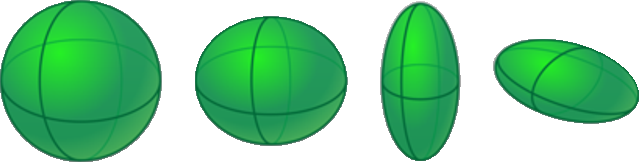
\includegraphics[width=.8\textwidth]{Shapes.pdf}
	\end{textblock*}

\end{frame}
\end{SectionTitle}

\begin{frame}{Setting up the calculations}
    \begin{textblock*}{0.45\paperwidth}(0.05\paperwidth,0.18\paperheight)
        \centering
        \only<1>{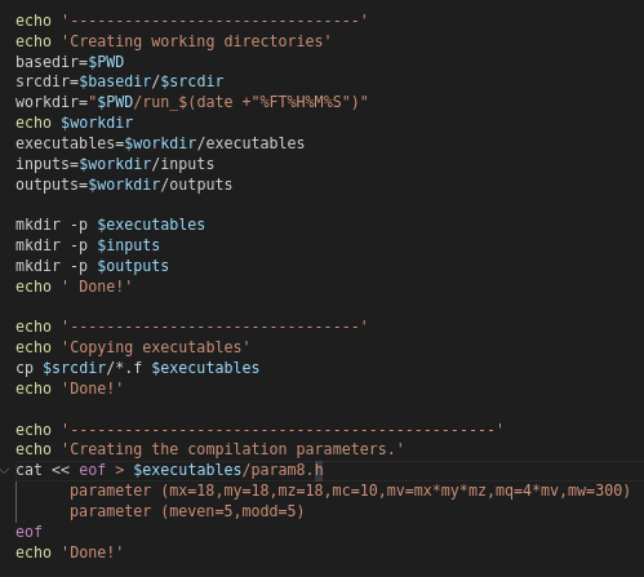
\includegraphics[width=1.\textwidth]{initialization.png}}%
        \only<2>{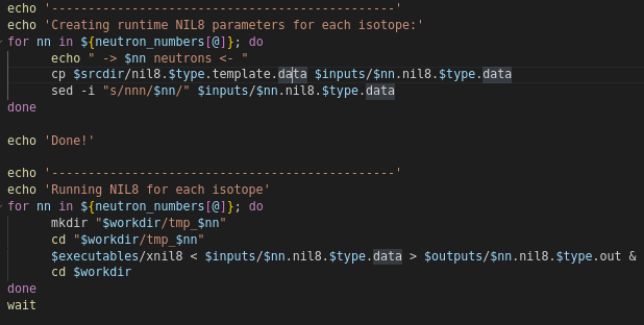
\includegraphics[width=1.\textwidth]{nil8compile.png}}%
        \only<3>{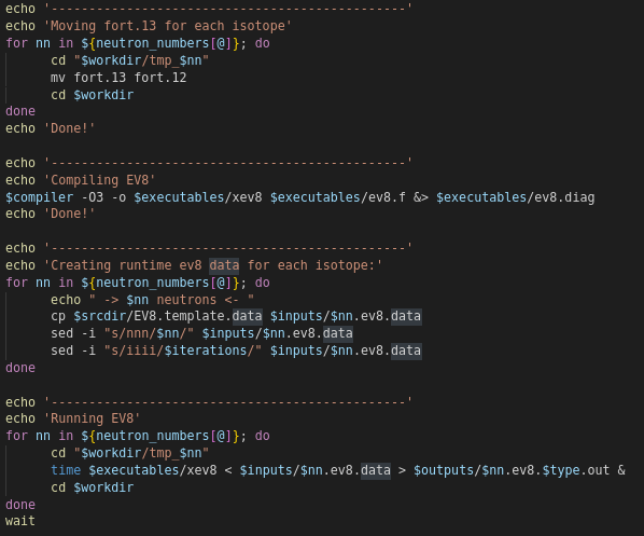
\includegraphics[width=1.\textwidth]{ev8run.png}}%
    \end{textblock*}
    \begin{textblock*}{0.45\paperwidth}(0.5\paperwidth,0.18\paperheight)
        \centering
        \small
        \begin{itemize}
            \item<1-> Creation of working directories and move of the source files into them. 
            \item<1-> Creation of param8.h input file
            \item<2-> Creation of a temporary directory for each isotope
            \item<2-> Copy of the nil8 template data file into each folder and substitution of the neutron number 
            \item<2-> nil8 parallel execution
            \item<3-> Same as before but for ev8
        \end{itemize}
    \end{textblock*}
\end{frame}

\begin{frame}{$^{238}$U EV8 calculations - Iterations}
    \centering 
    \begin{textblock*}{0.5\paperwidth}(0.\paperwidth,0.2\paperheight)
        \centering
        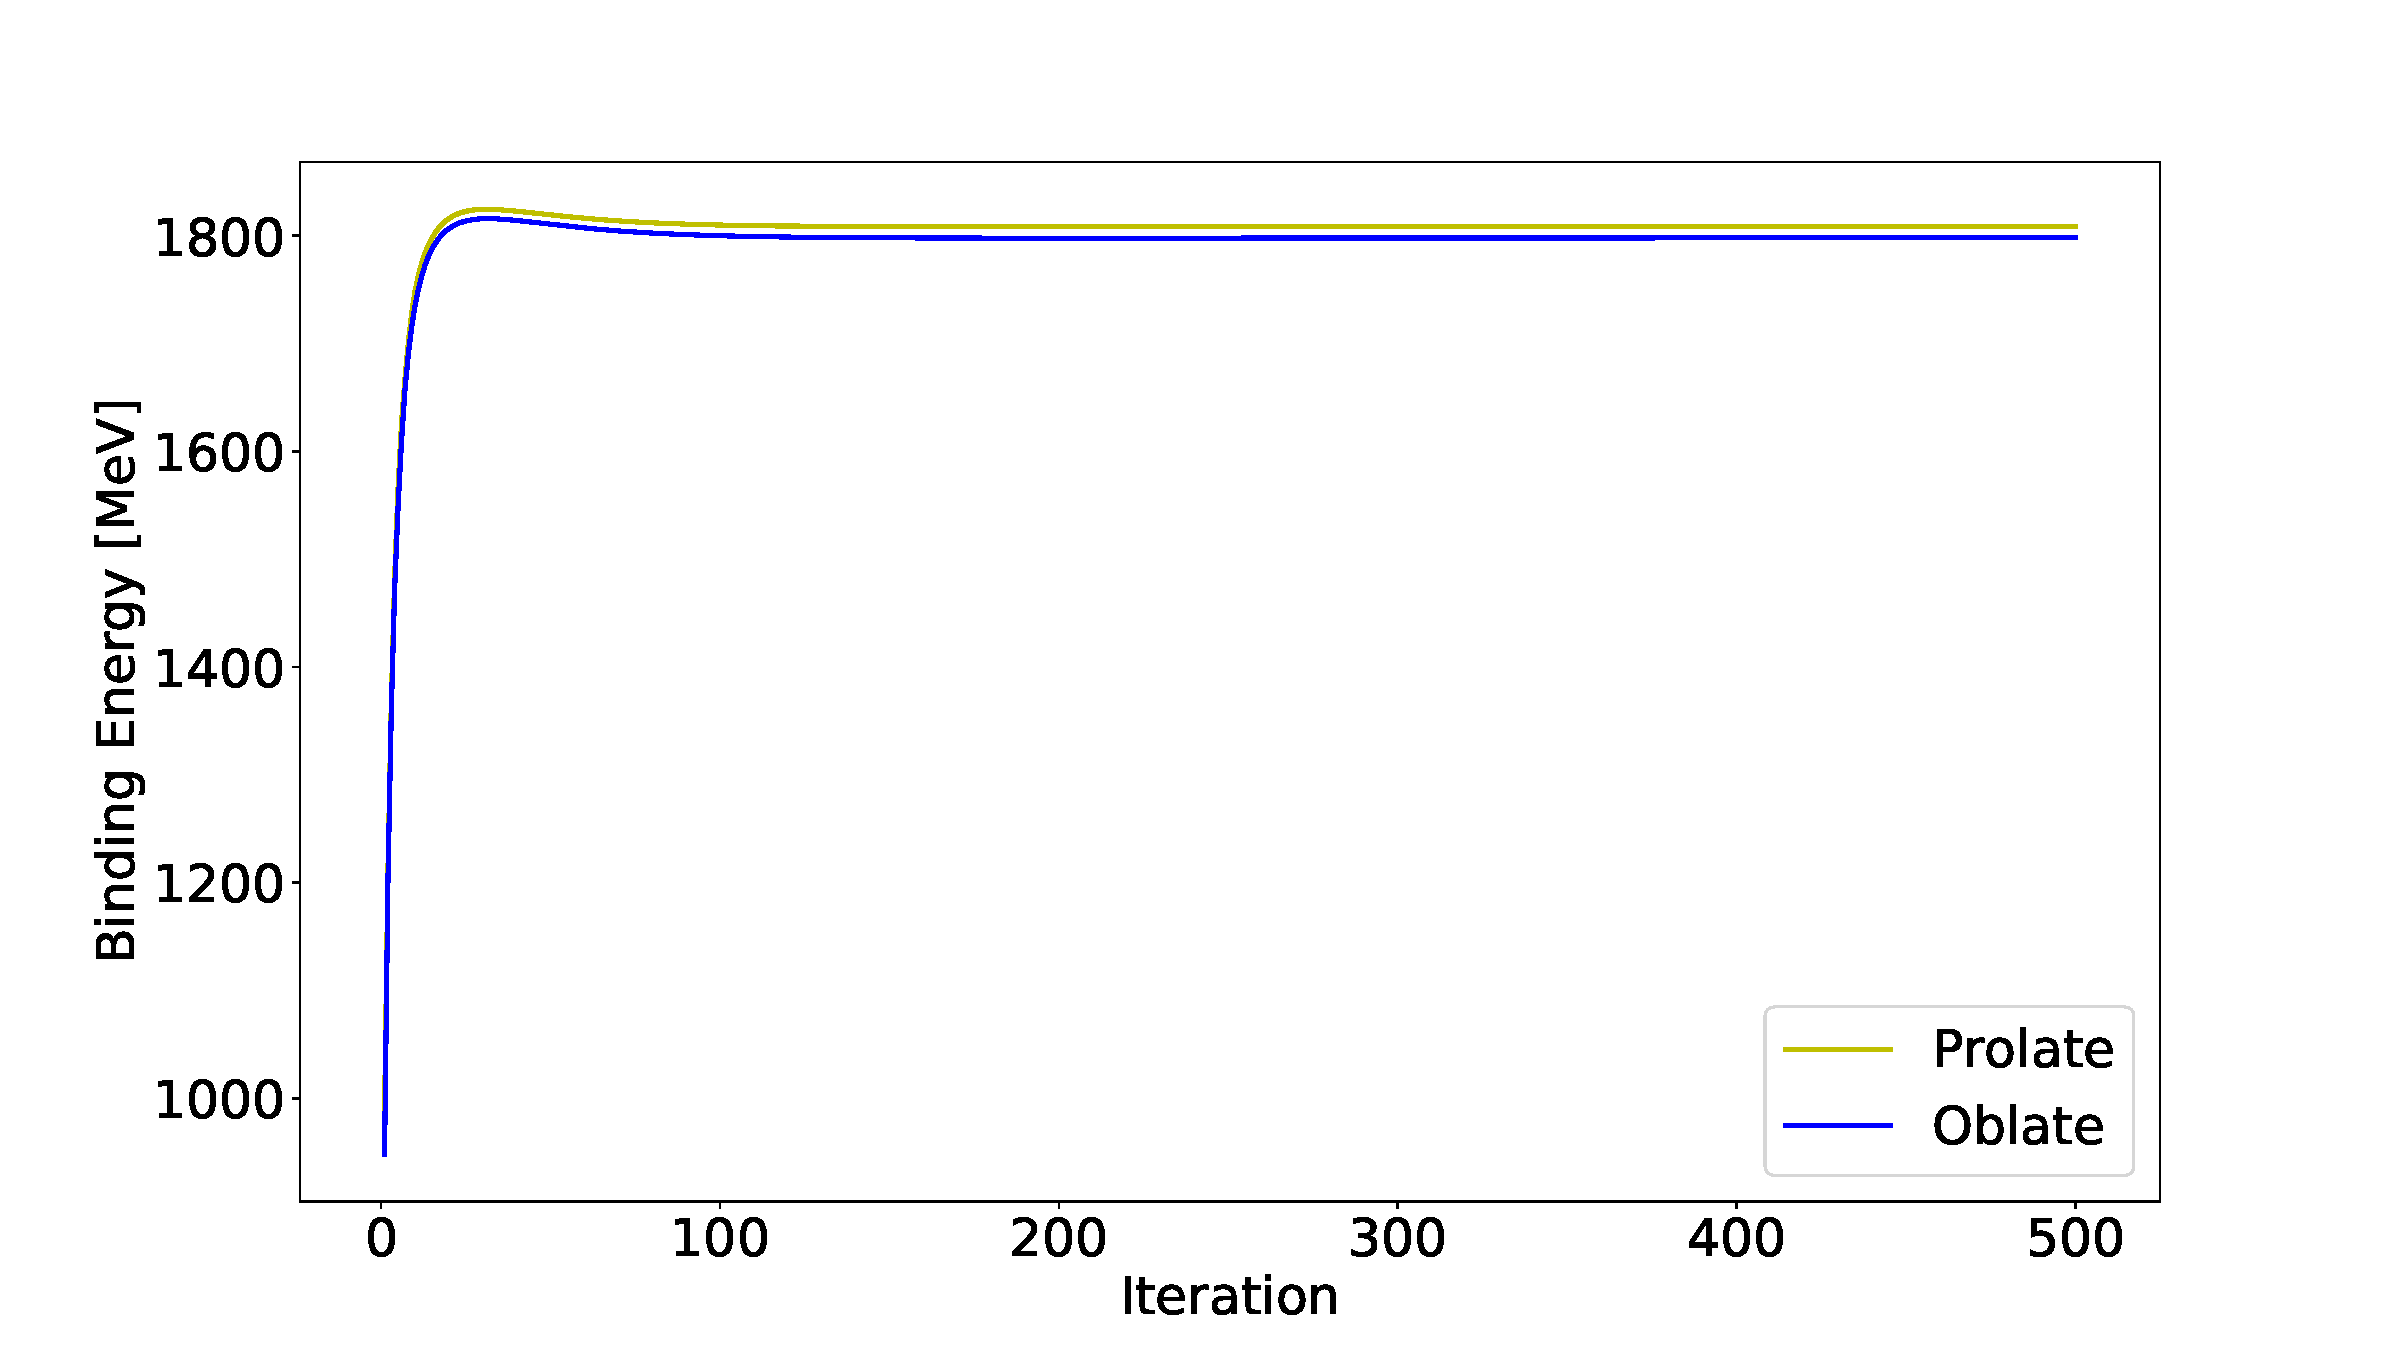
\includegraphics[width=1.1\textwidth]{iteration.pdf}
    \end{textblock*}
    \begin{textblock*}{0.5\paperwidth}(0.48\paperwidth,0.2\paperheight)
        \centering
        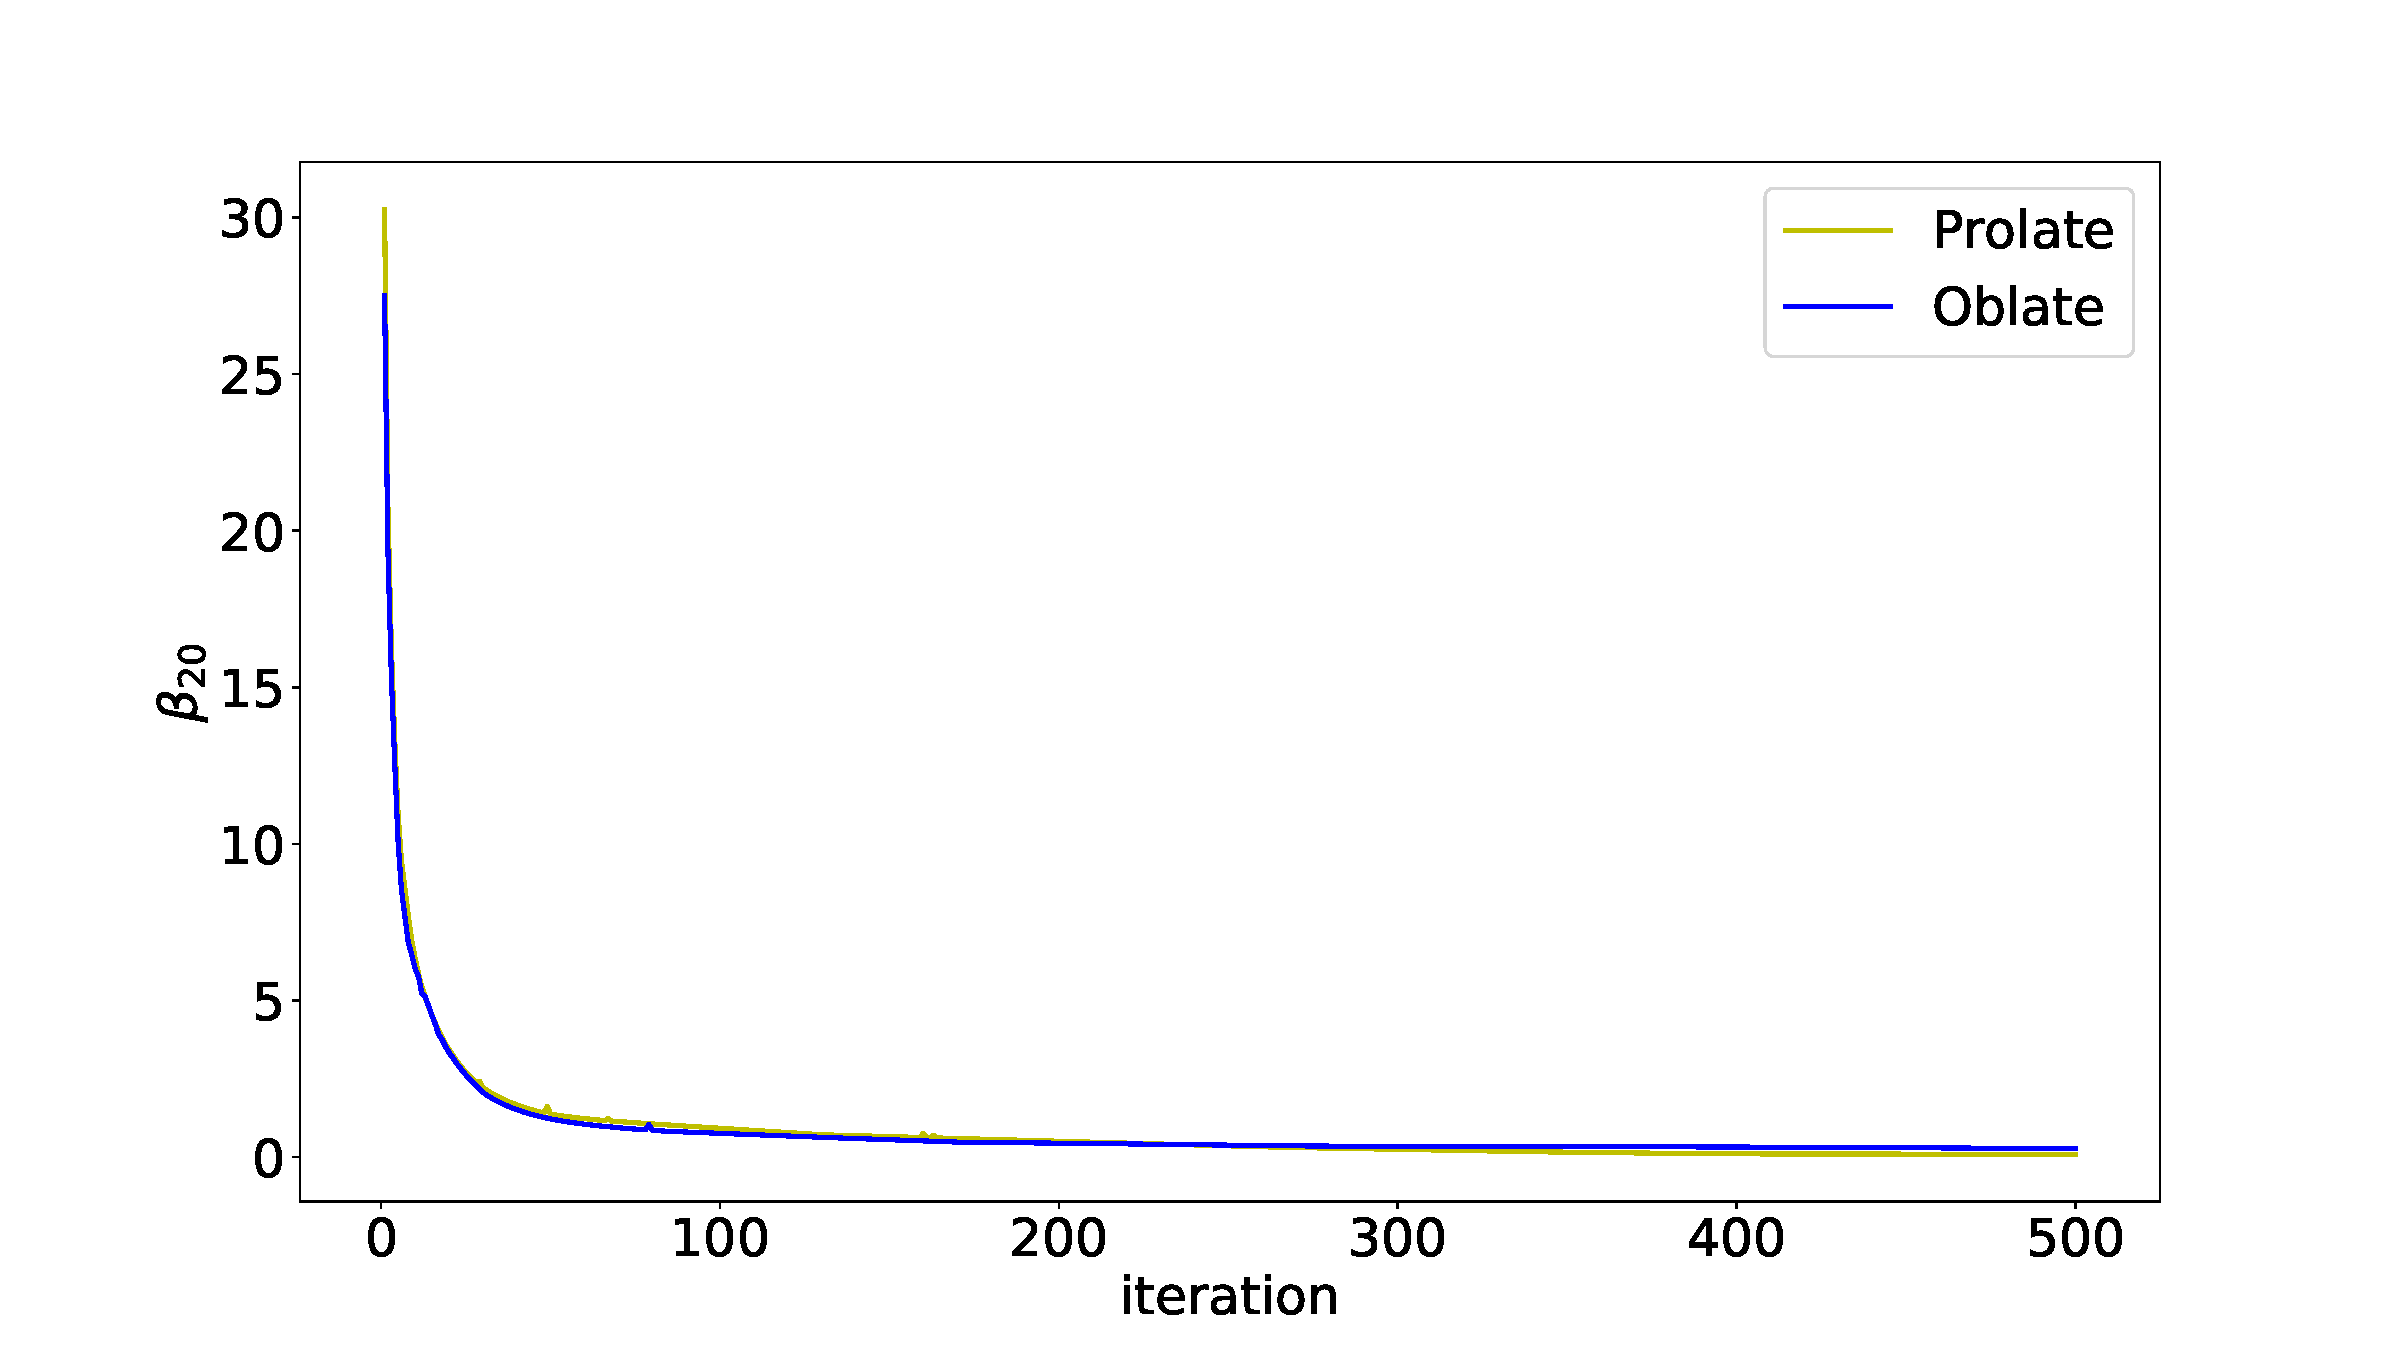
\includegraphics[width=1.1\textwidth]{iterationB20.pdf}
    \end{textblock*}
    \begin{textblock*}{0.8\paperwidth}(0.1\paperwidth,0.8\paperheight)
        \centering
        After few 100s iteration the calculations start to converge. All following plots are obtained with 500 iterations calculations.
    \end{textblock*}
\end{frame}

\begin{frame}{Binding energies}

    \centering 
    \begin{textblock*}{0.8\paperwidth}(0.1\paperwidth,0.22\paperheight)
        \centering
        Binding energy difference between prolate and oblate deformations
    \end{textblock*}
    \begin{textblock*}{0.5\paperwidth}(0.\paperwidth,0.25\paperheight)
        \centering
        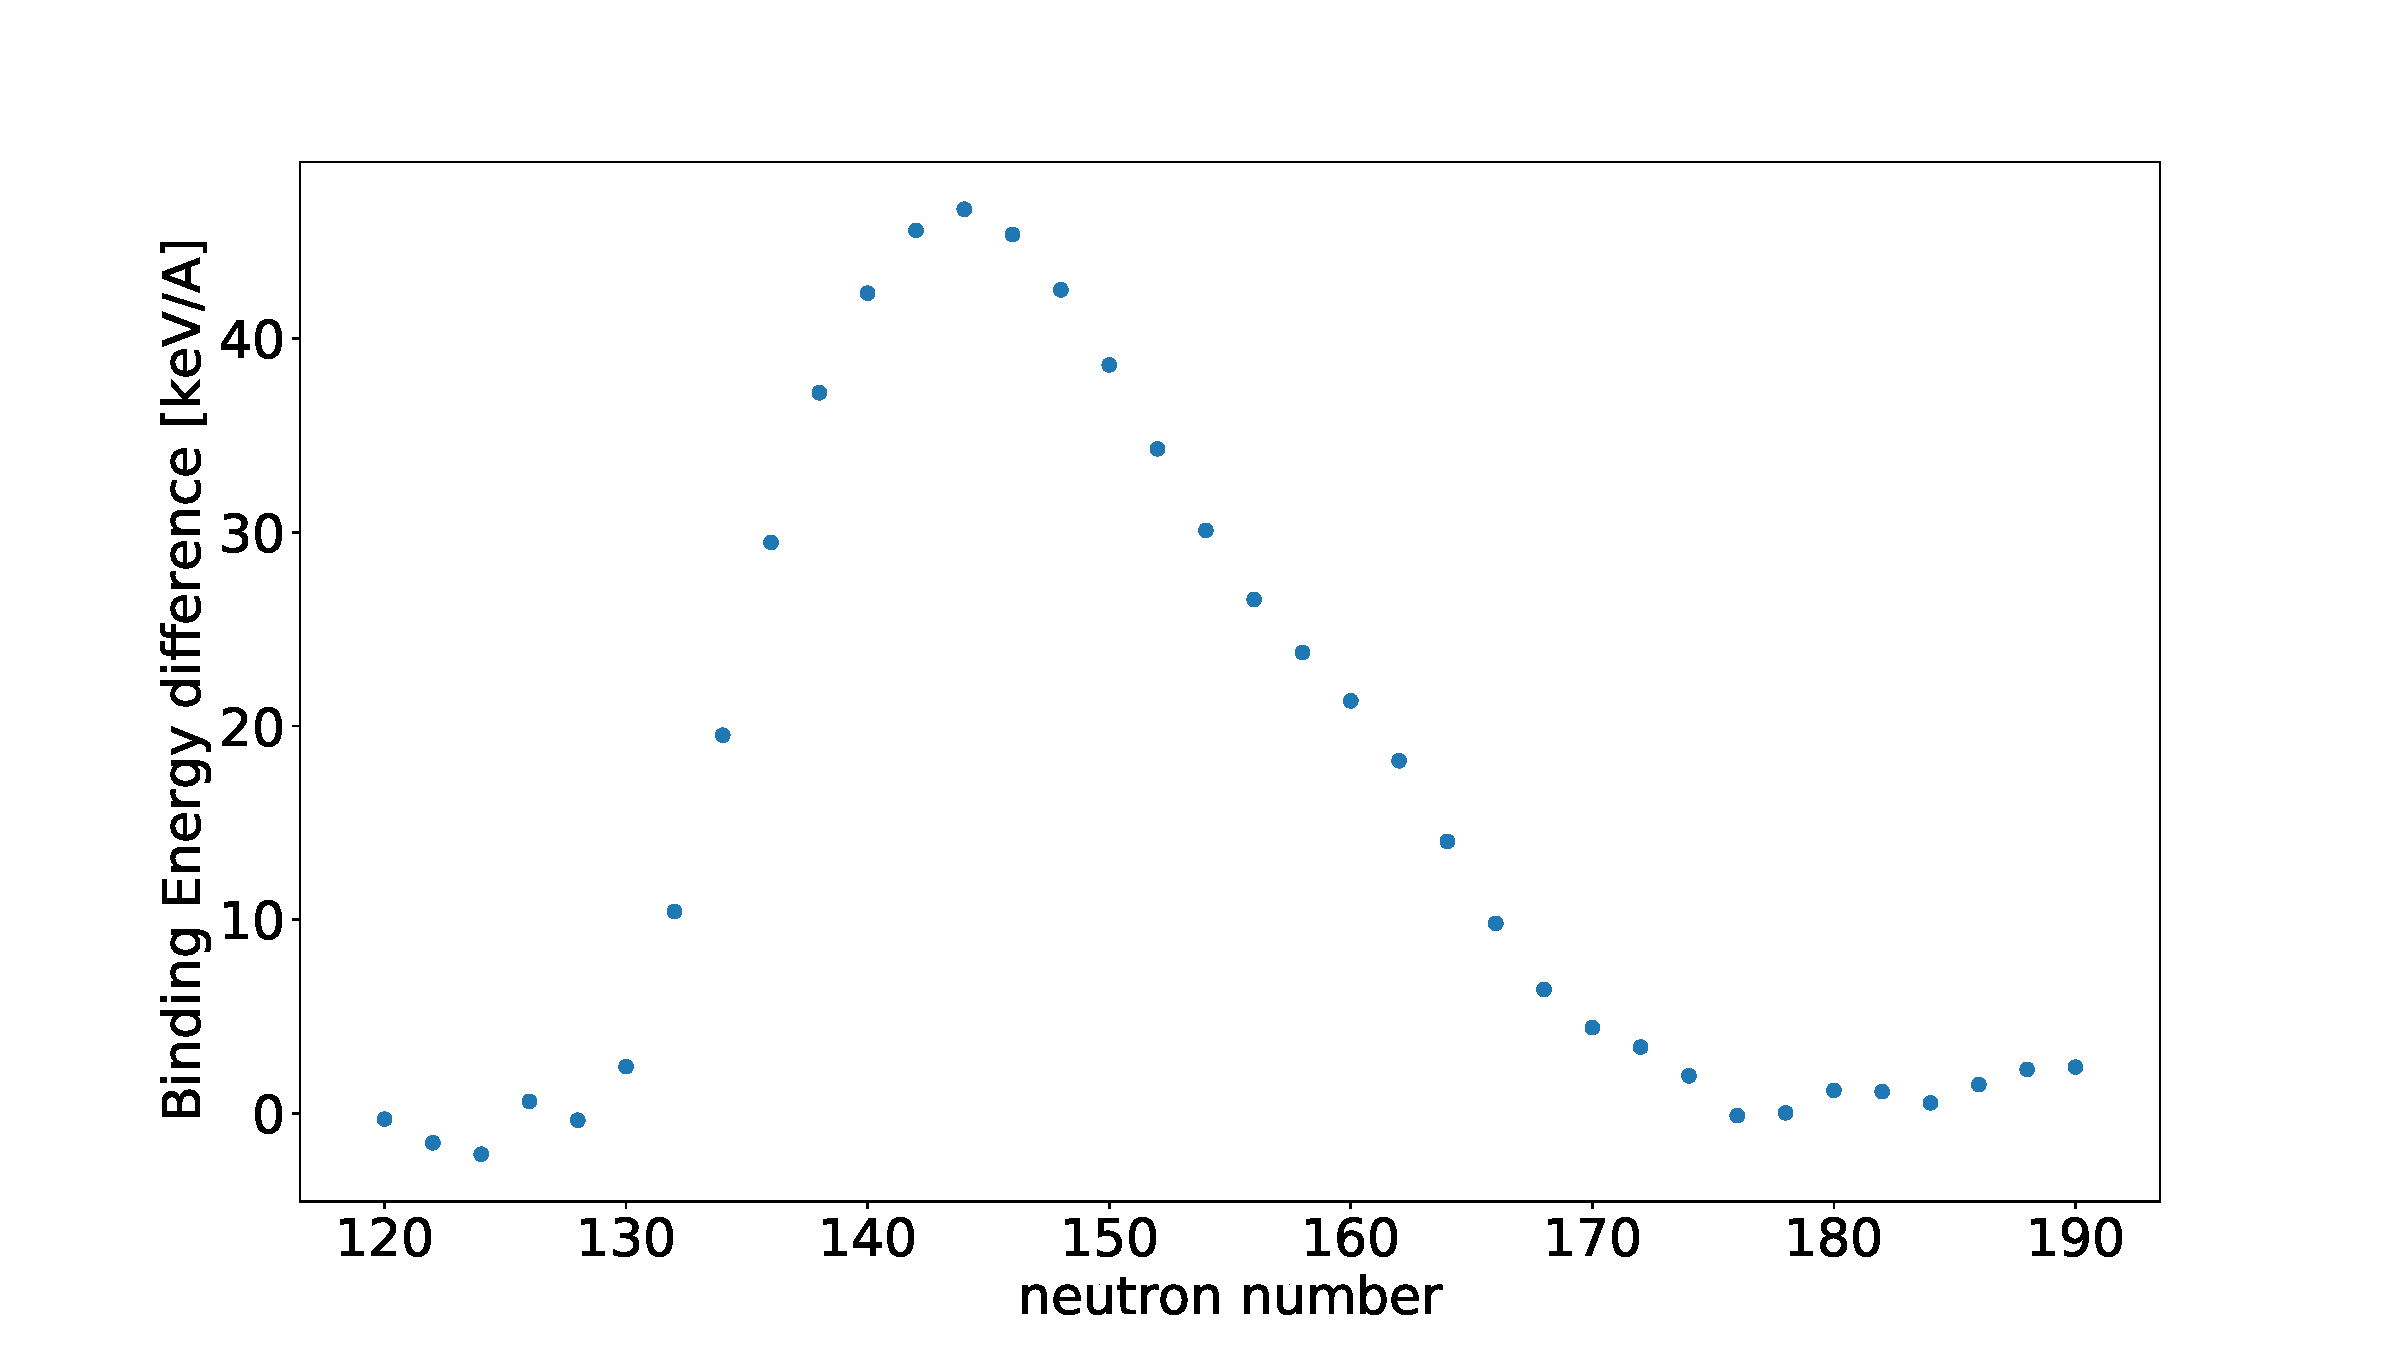
\includegraphics[width=1.1\textwidth]{bindingenergies.pdf}
    \end{textblock*}
    \begin{textblock*}{0.45\paperwidth}(0.5\paperwidth,0.35\paperheight)
        % \centering
        \only<1>{
            \centering
            \textbf{$^{238}$U}\\
            \textbf{Prolate}\\
            Binding energy = 7520.3 [keV/A]\\
            \textbf{Oblate}\\
            Binding energy = 7474.9 [keV/A]\\
            \textbf{Experiment}\\
            Binding energy = 7570.126(6) [keV/A] \footnote<1>{Nuclear Data Sheets 127, 191 (2015)}
        }
        \only<2>{
            \begin{itemize}
                \item Positive difference means that the prolate configuration is preferred with respect to the oblate one.
                \item At N=126 and N=174 the difference between the two configuration is smaller, this is because we are approaching neutron magic numbers, where the nuclues is supposed to be spherical.
            \end{itemize}
        }
    \end{textblock*}
\end{frame}

\begin{frame}{RMS and isotopes shift}

    \centering 

    \begin{textblock*}{0.5\paperwidth}(0.\paperwidth,0.2\paperheight)
        \centering
        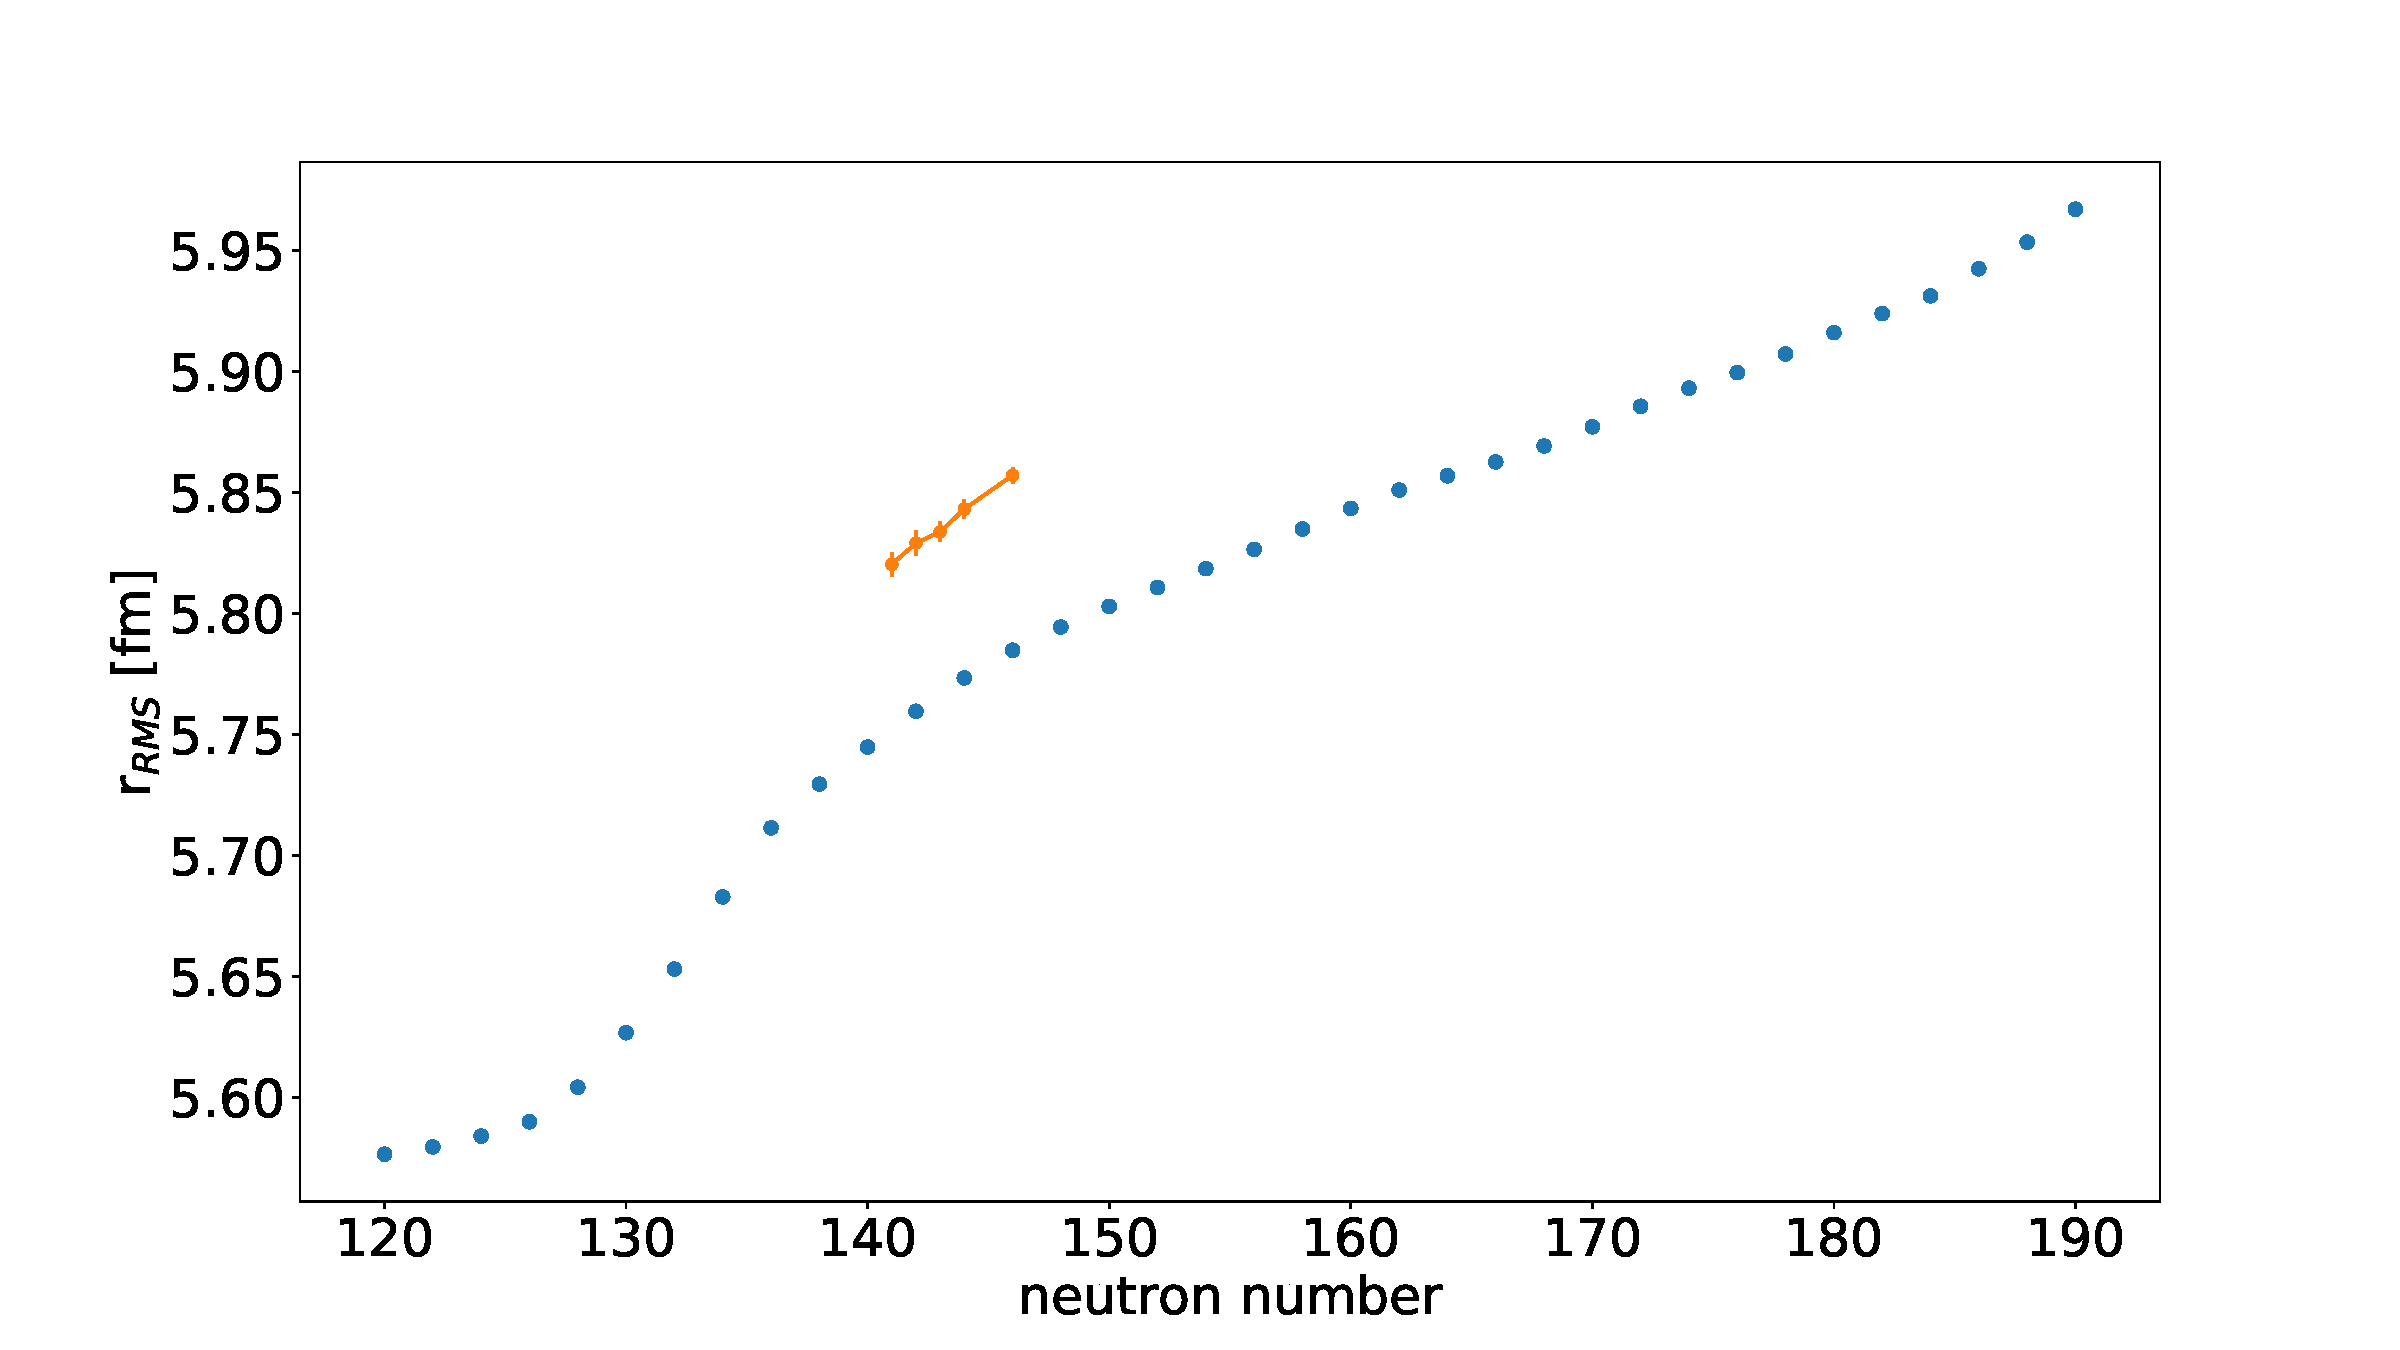
\includegraphics[width=1.1\textwidth]{rms.pdf}
    \end{textblock*}
    \begin{textblock*}{0.5\paperwidth}(0.48\paperwidth,0.2\paperheight)
        \centering
        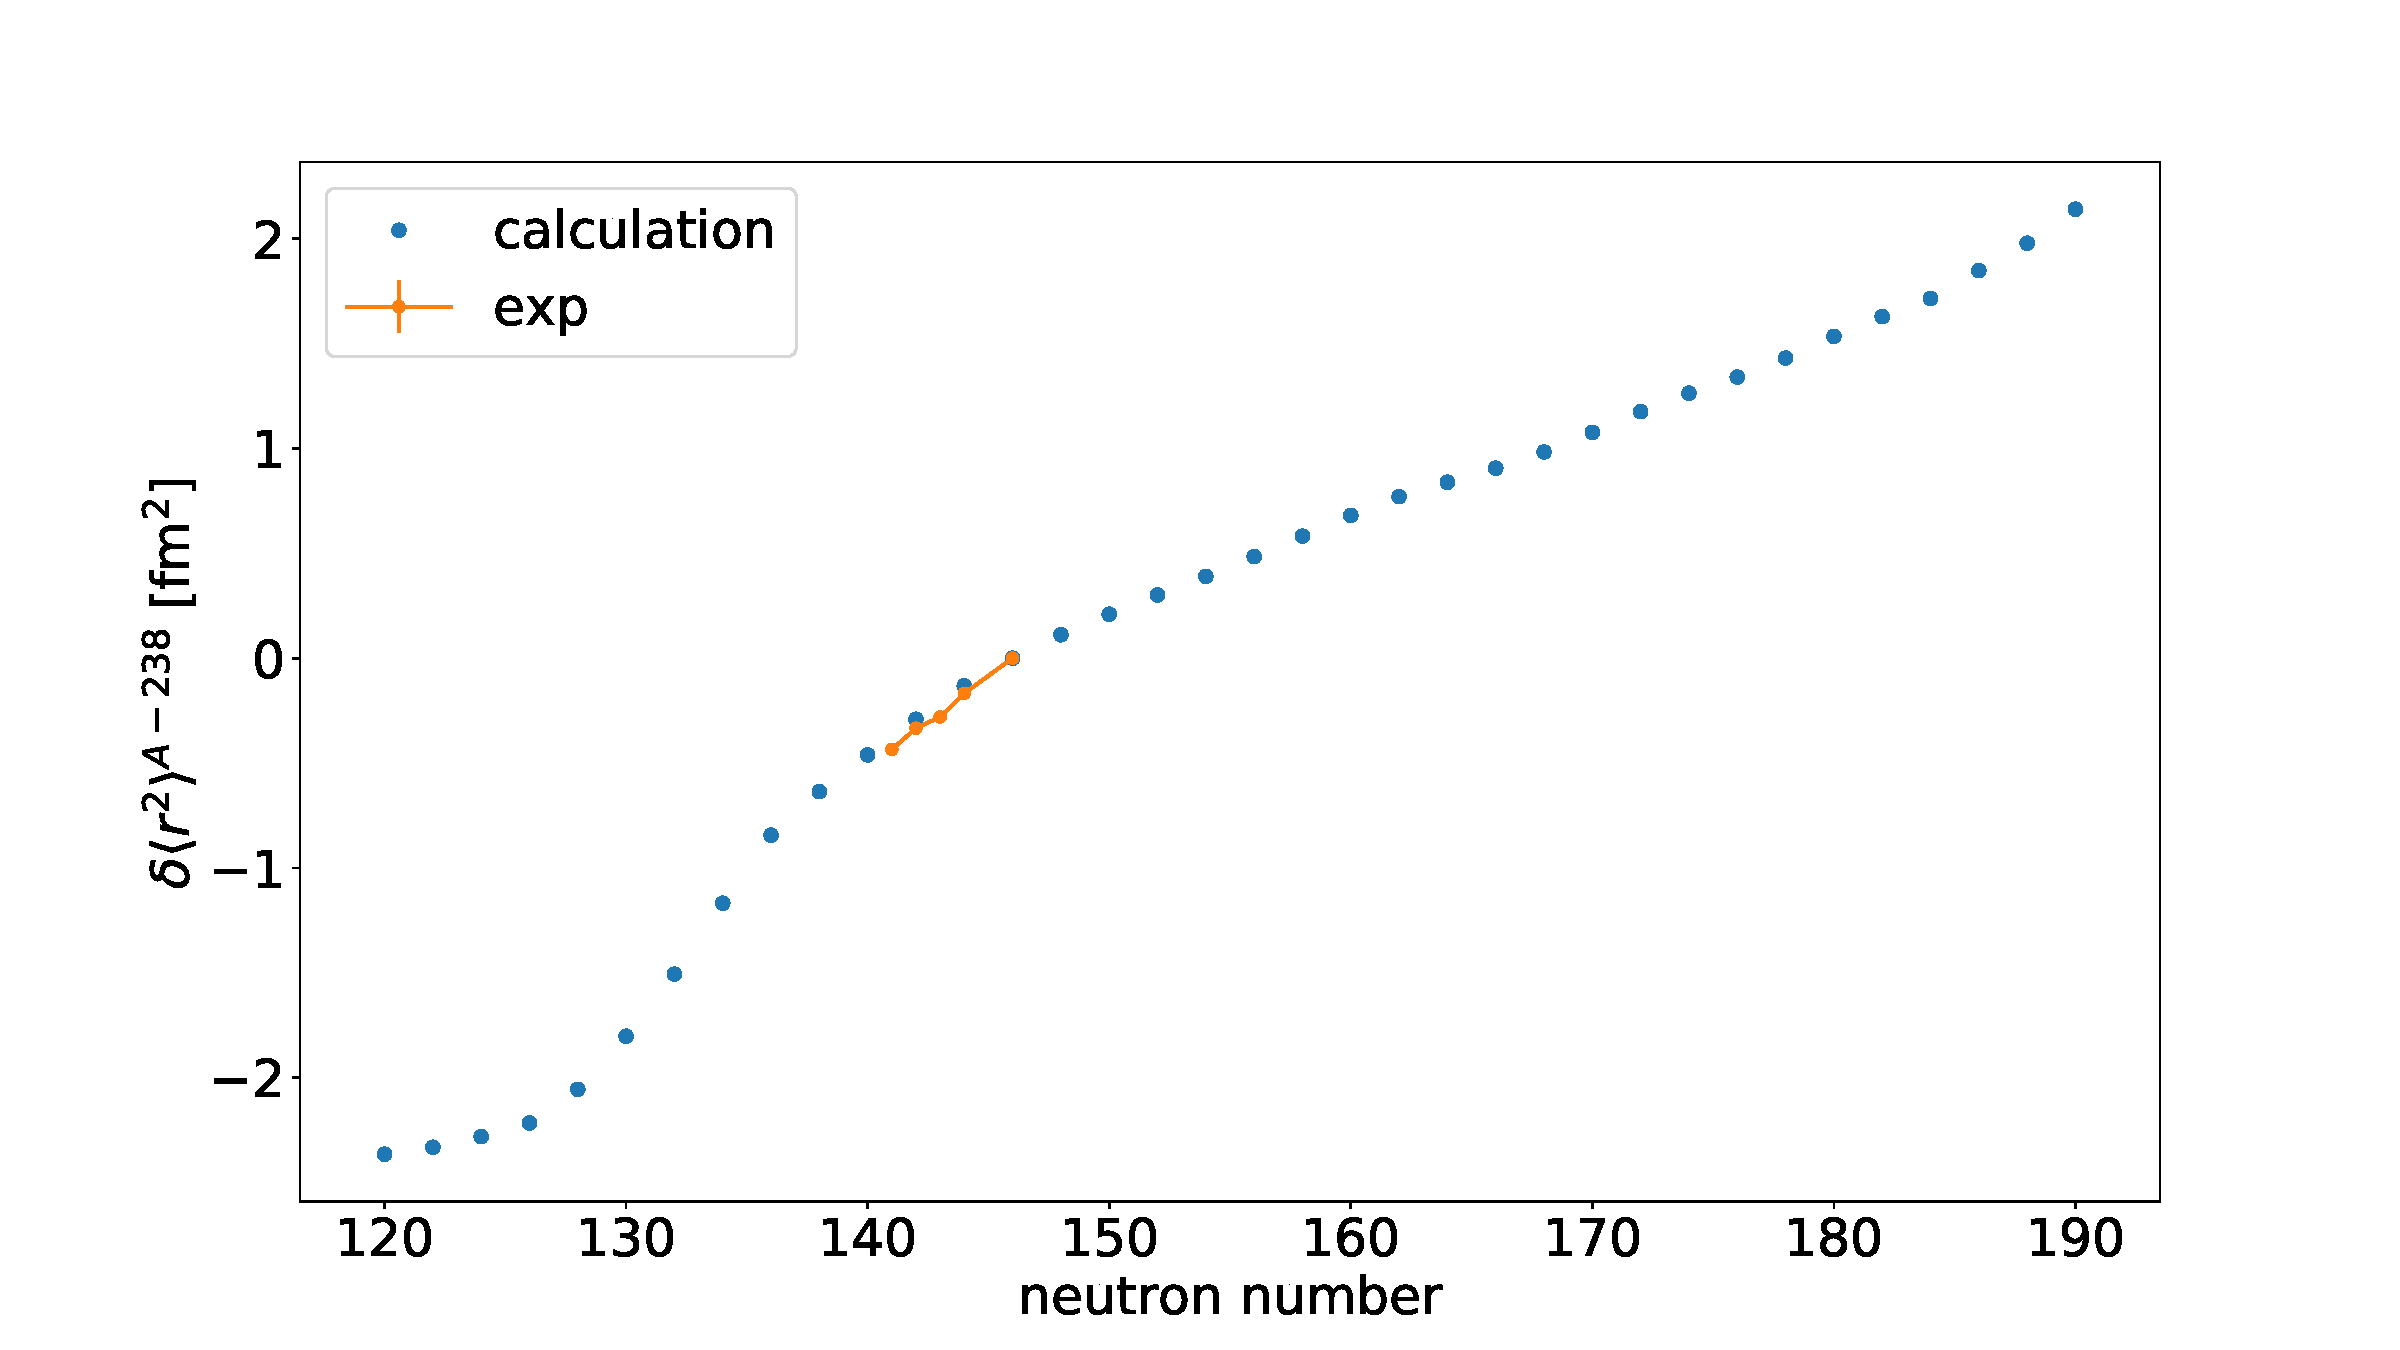
\includegraphics[width=1.1\textwidth]{ms.pdf}
    \end{textblock*}
    \begin{textblock*}{0.8\paperwidth}(0.1\paperwidth,0.8\paperheight)
        % \centering
        Proton finite size not considered, which explain why the computed rms is lower than the experimental value
    \end{textblock*}
\end{frame}


\begin{frame}{Quadrupole and higher order deformations}

    \centering 
    \begin{textblock*}{0.5\paperwidth}(0.\paperwidth,0.2\paperheight)
        \centering
        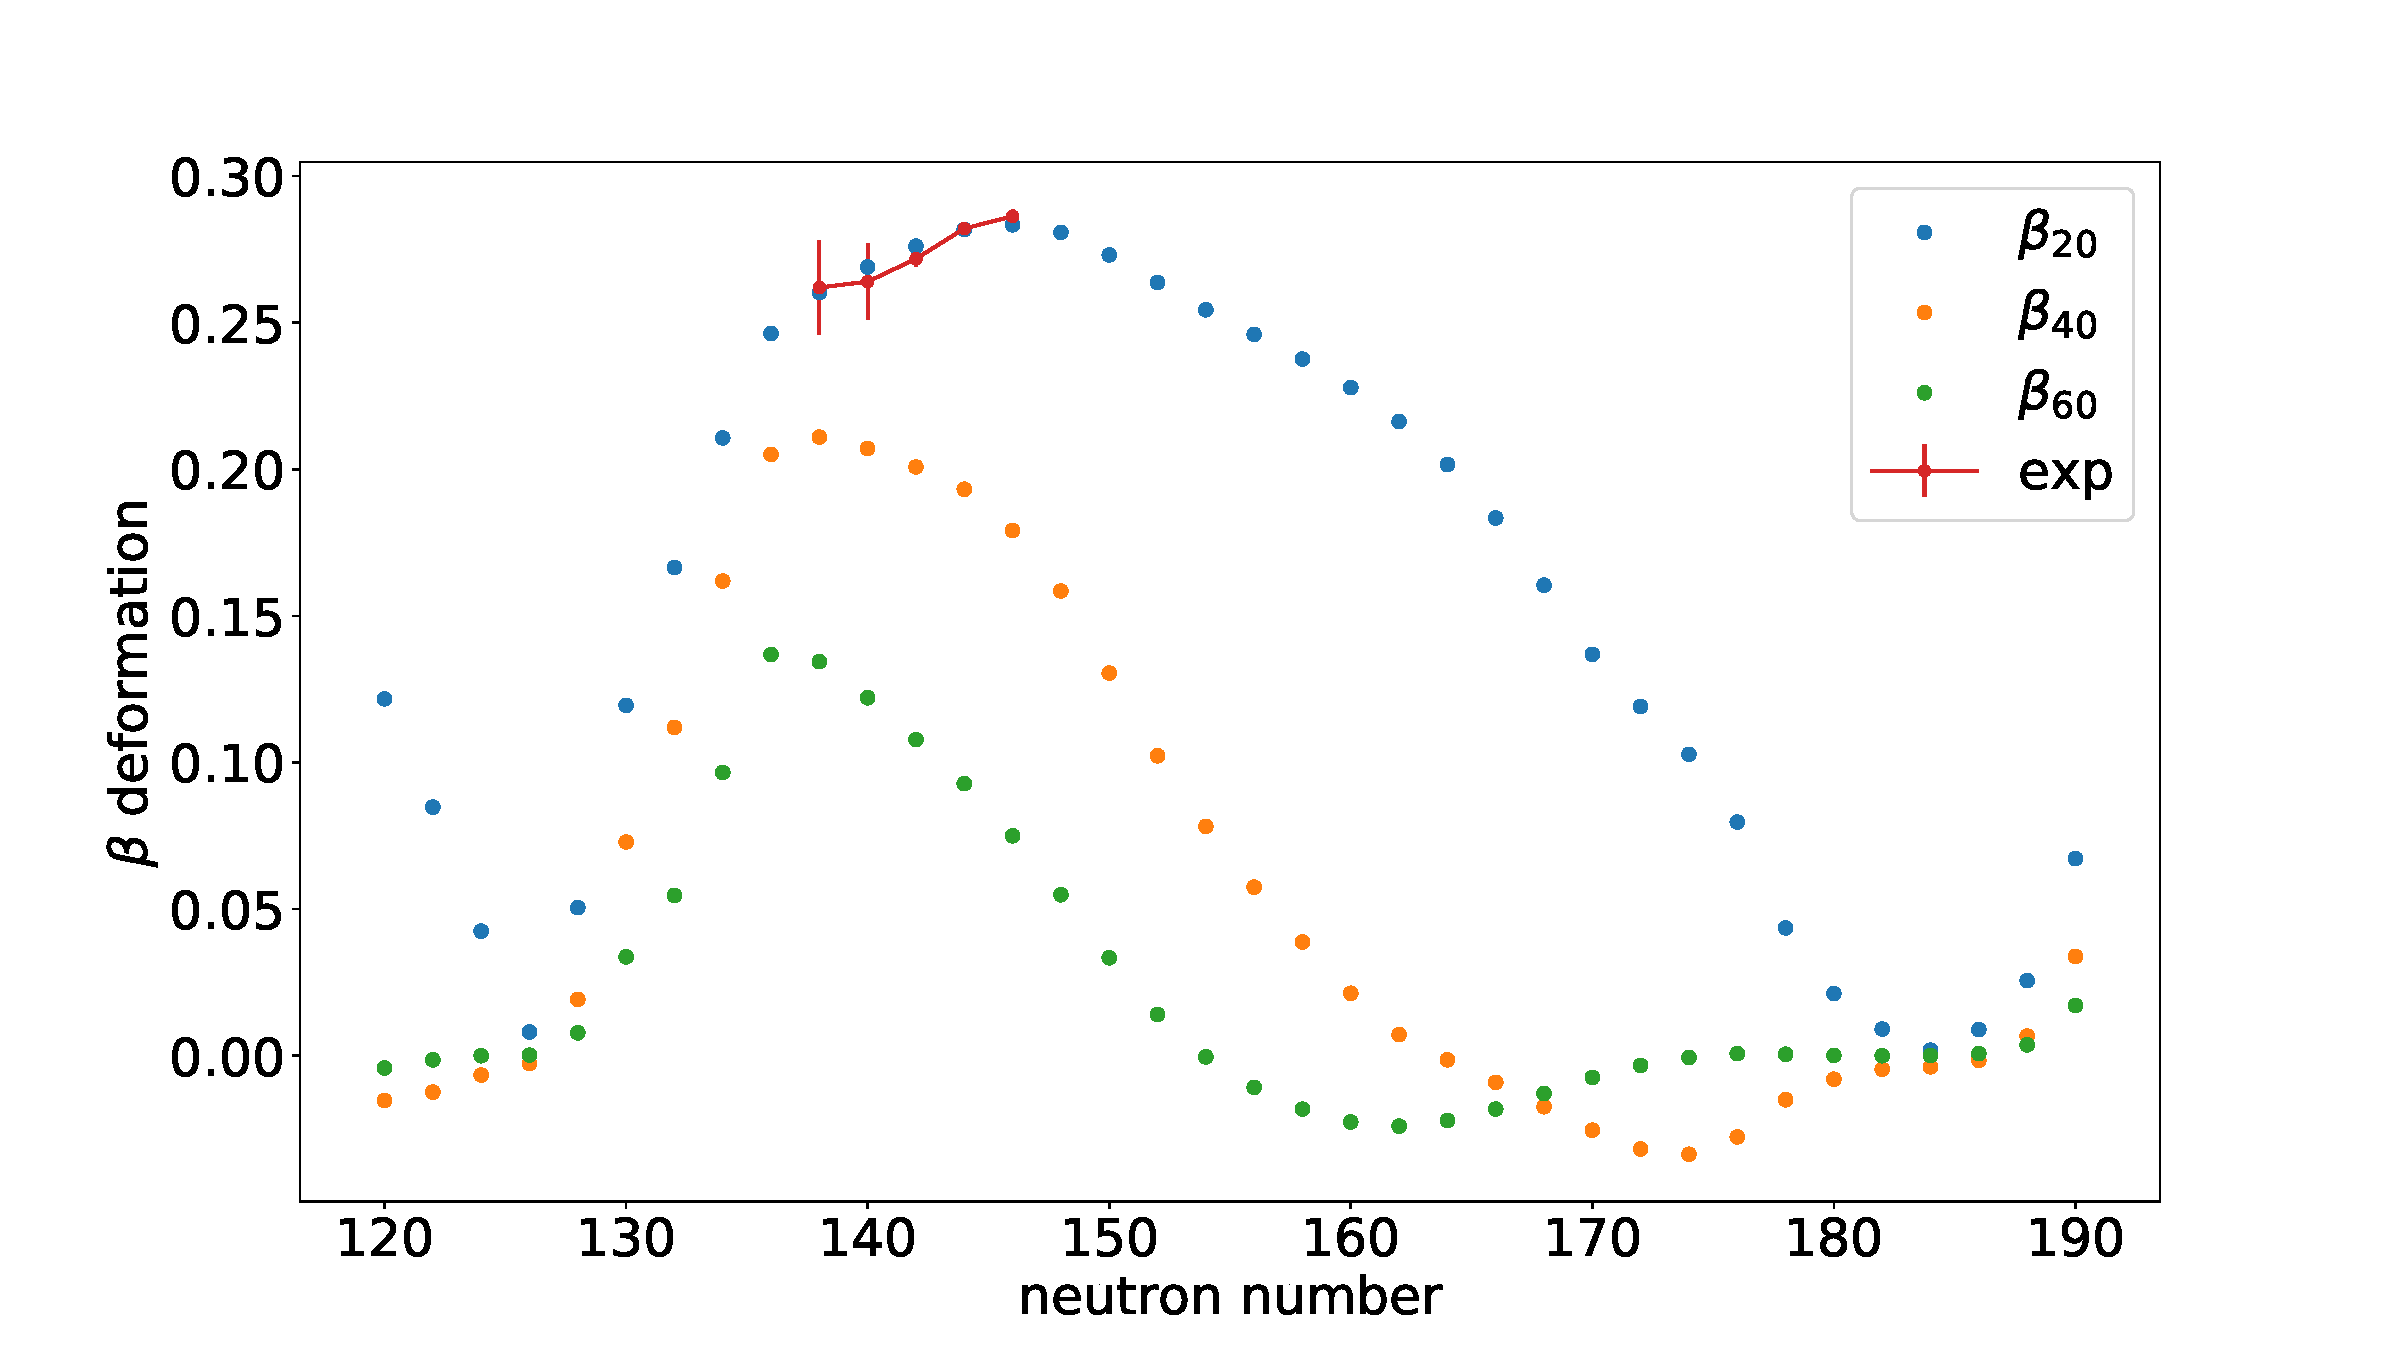
\includegraphics[width=1.1\textwidth]{beta.pdf}
    \end{textblock*}
    \begin{textblock*}{0.5\paperwidth}(0.48\paperwidth,0.2\paperheight)
        % \centering
        \only<1>{
            \centering
            \vspace{0.2\textheight}
            \begin{itemize}
                \item Quadrupole deformation is well reproduced by the calculations
                \item $\beta_{40}$ and $\beta_{60}$ contribute in theory but $\beta_{20}$ dominate the rms in practice.
            \end{itemize}
        }
        \only<2>{
            \centering
            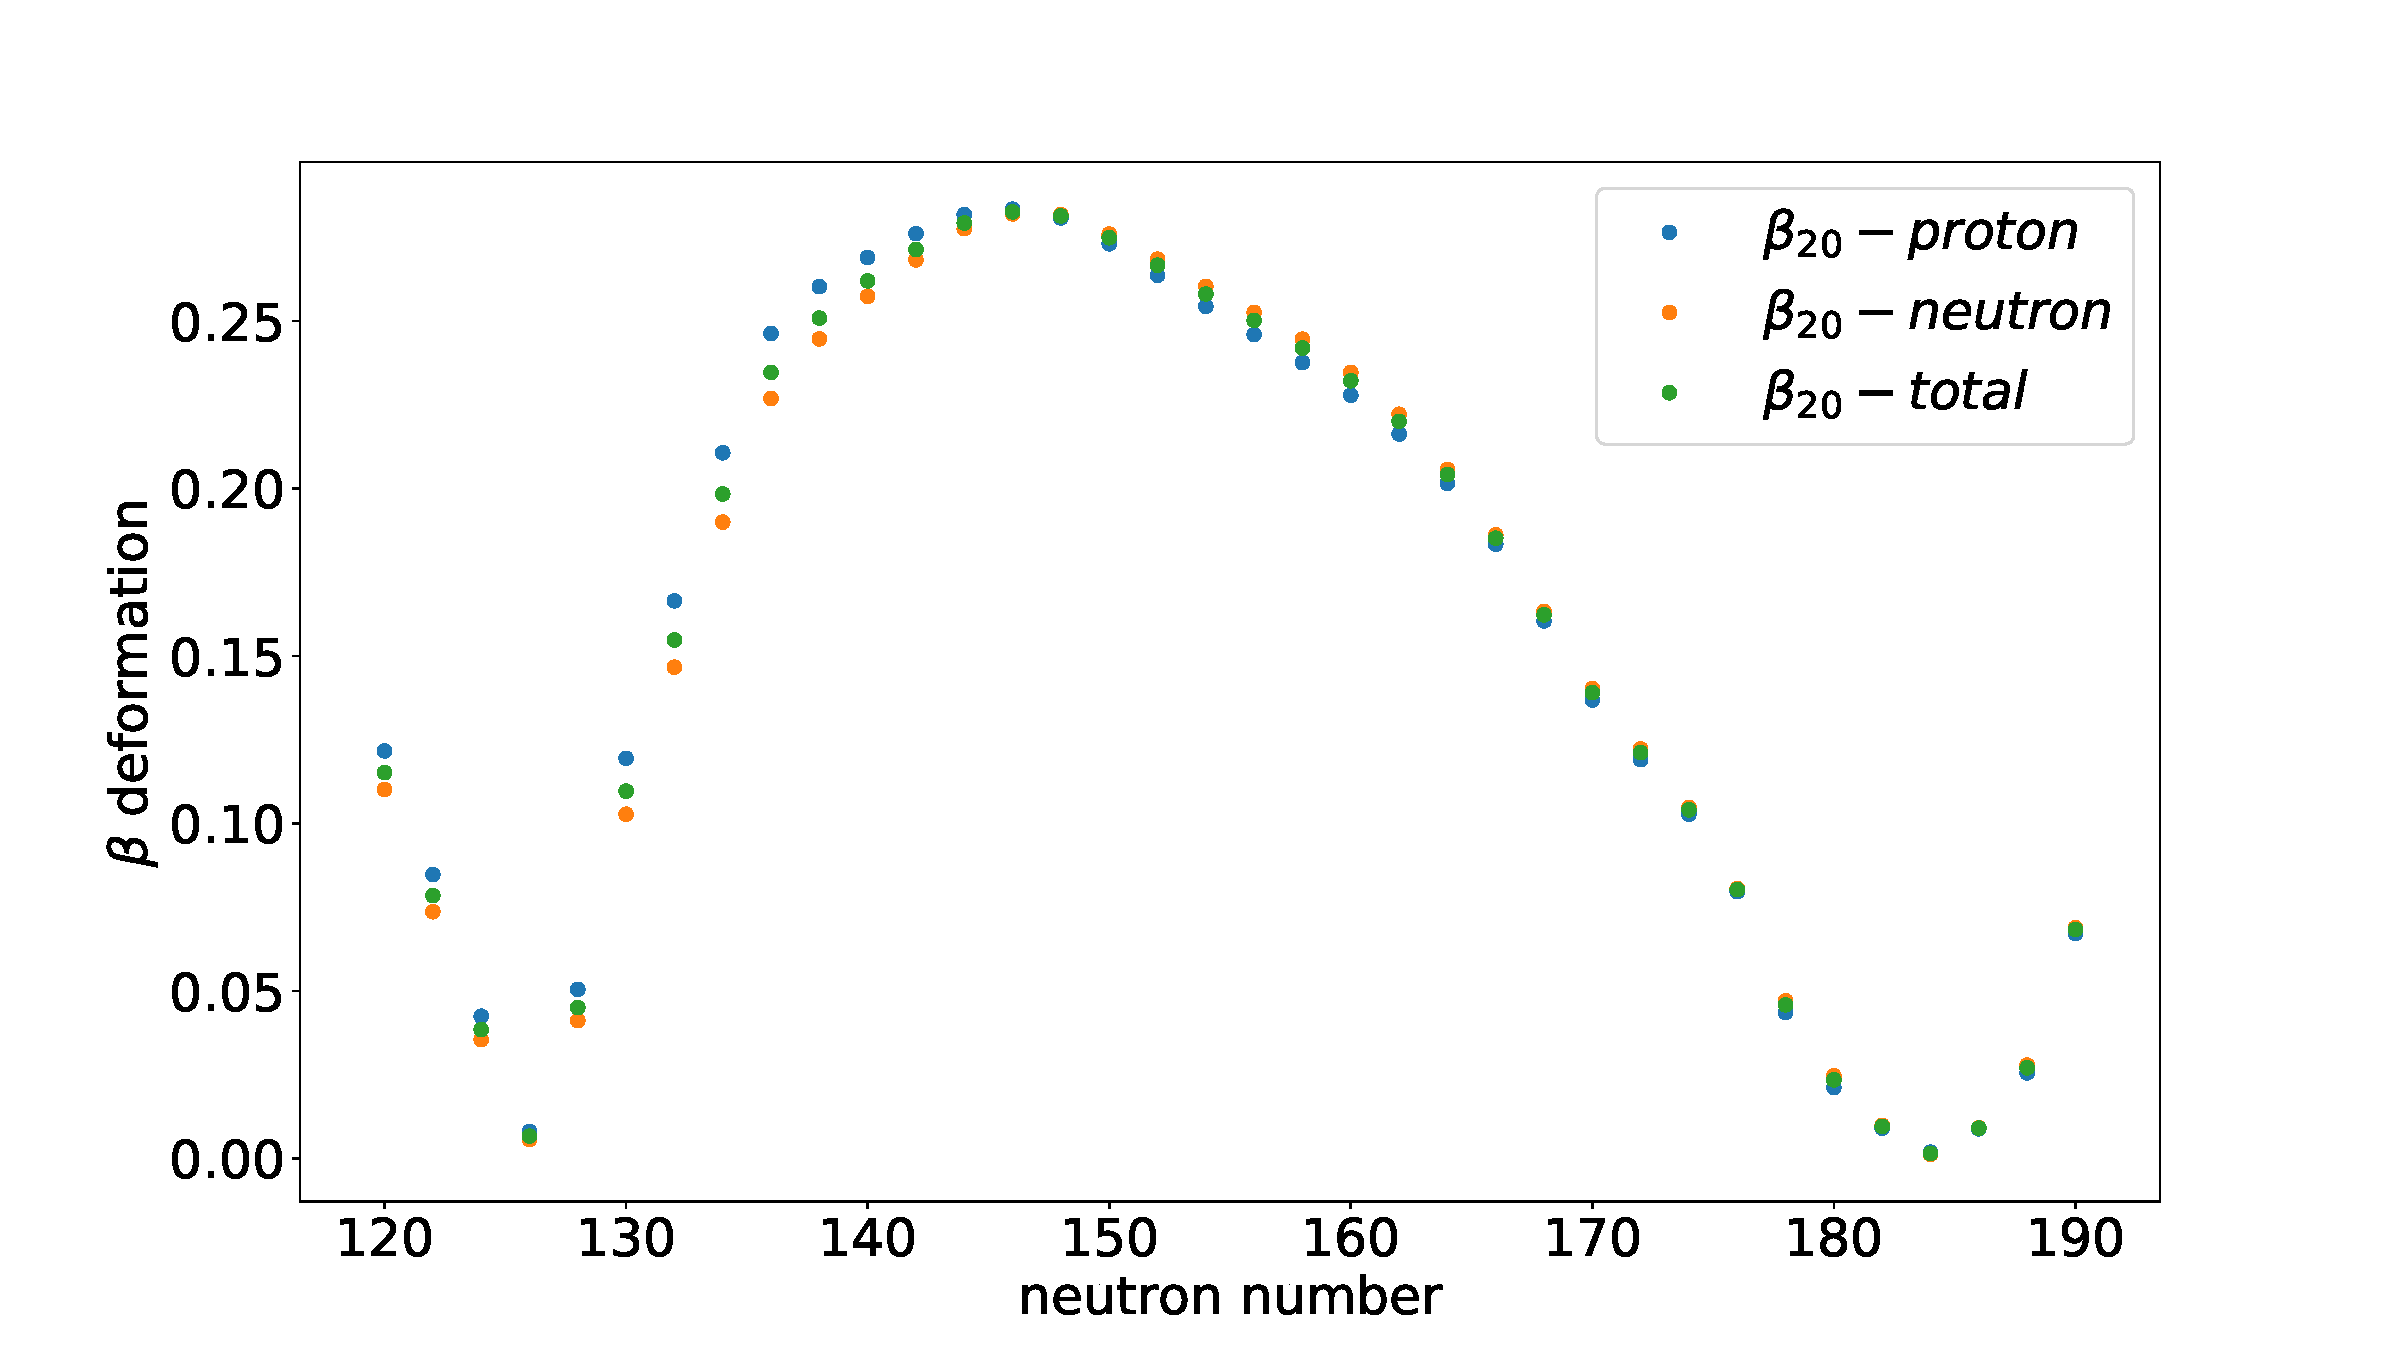
\includegraphics[width=1.1\textwidth]{beta_comp.pdf}
        }

    \end{textblock*}
\end{frame}


\begin{frame}{Neutron skin}

    \centering 
    \begin{textblock*}{0.5\paperwidth}(0.\paperwidth,0.3\paperheight)
        \centering
        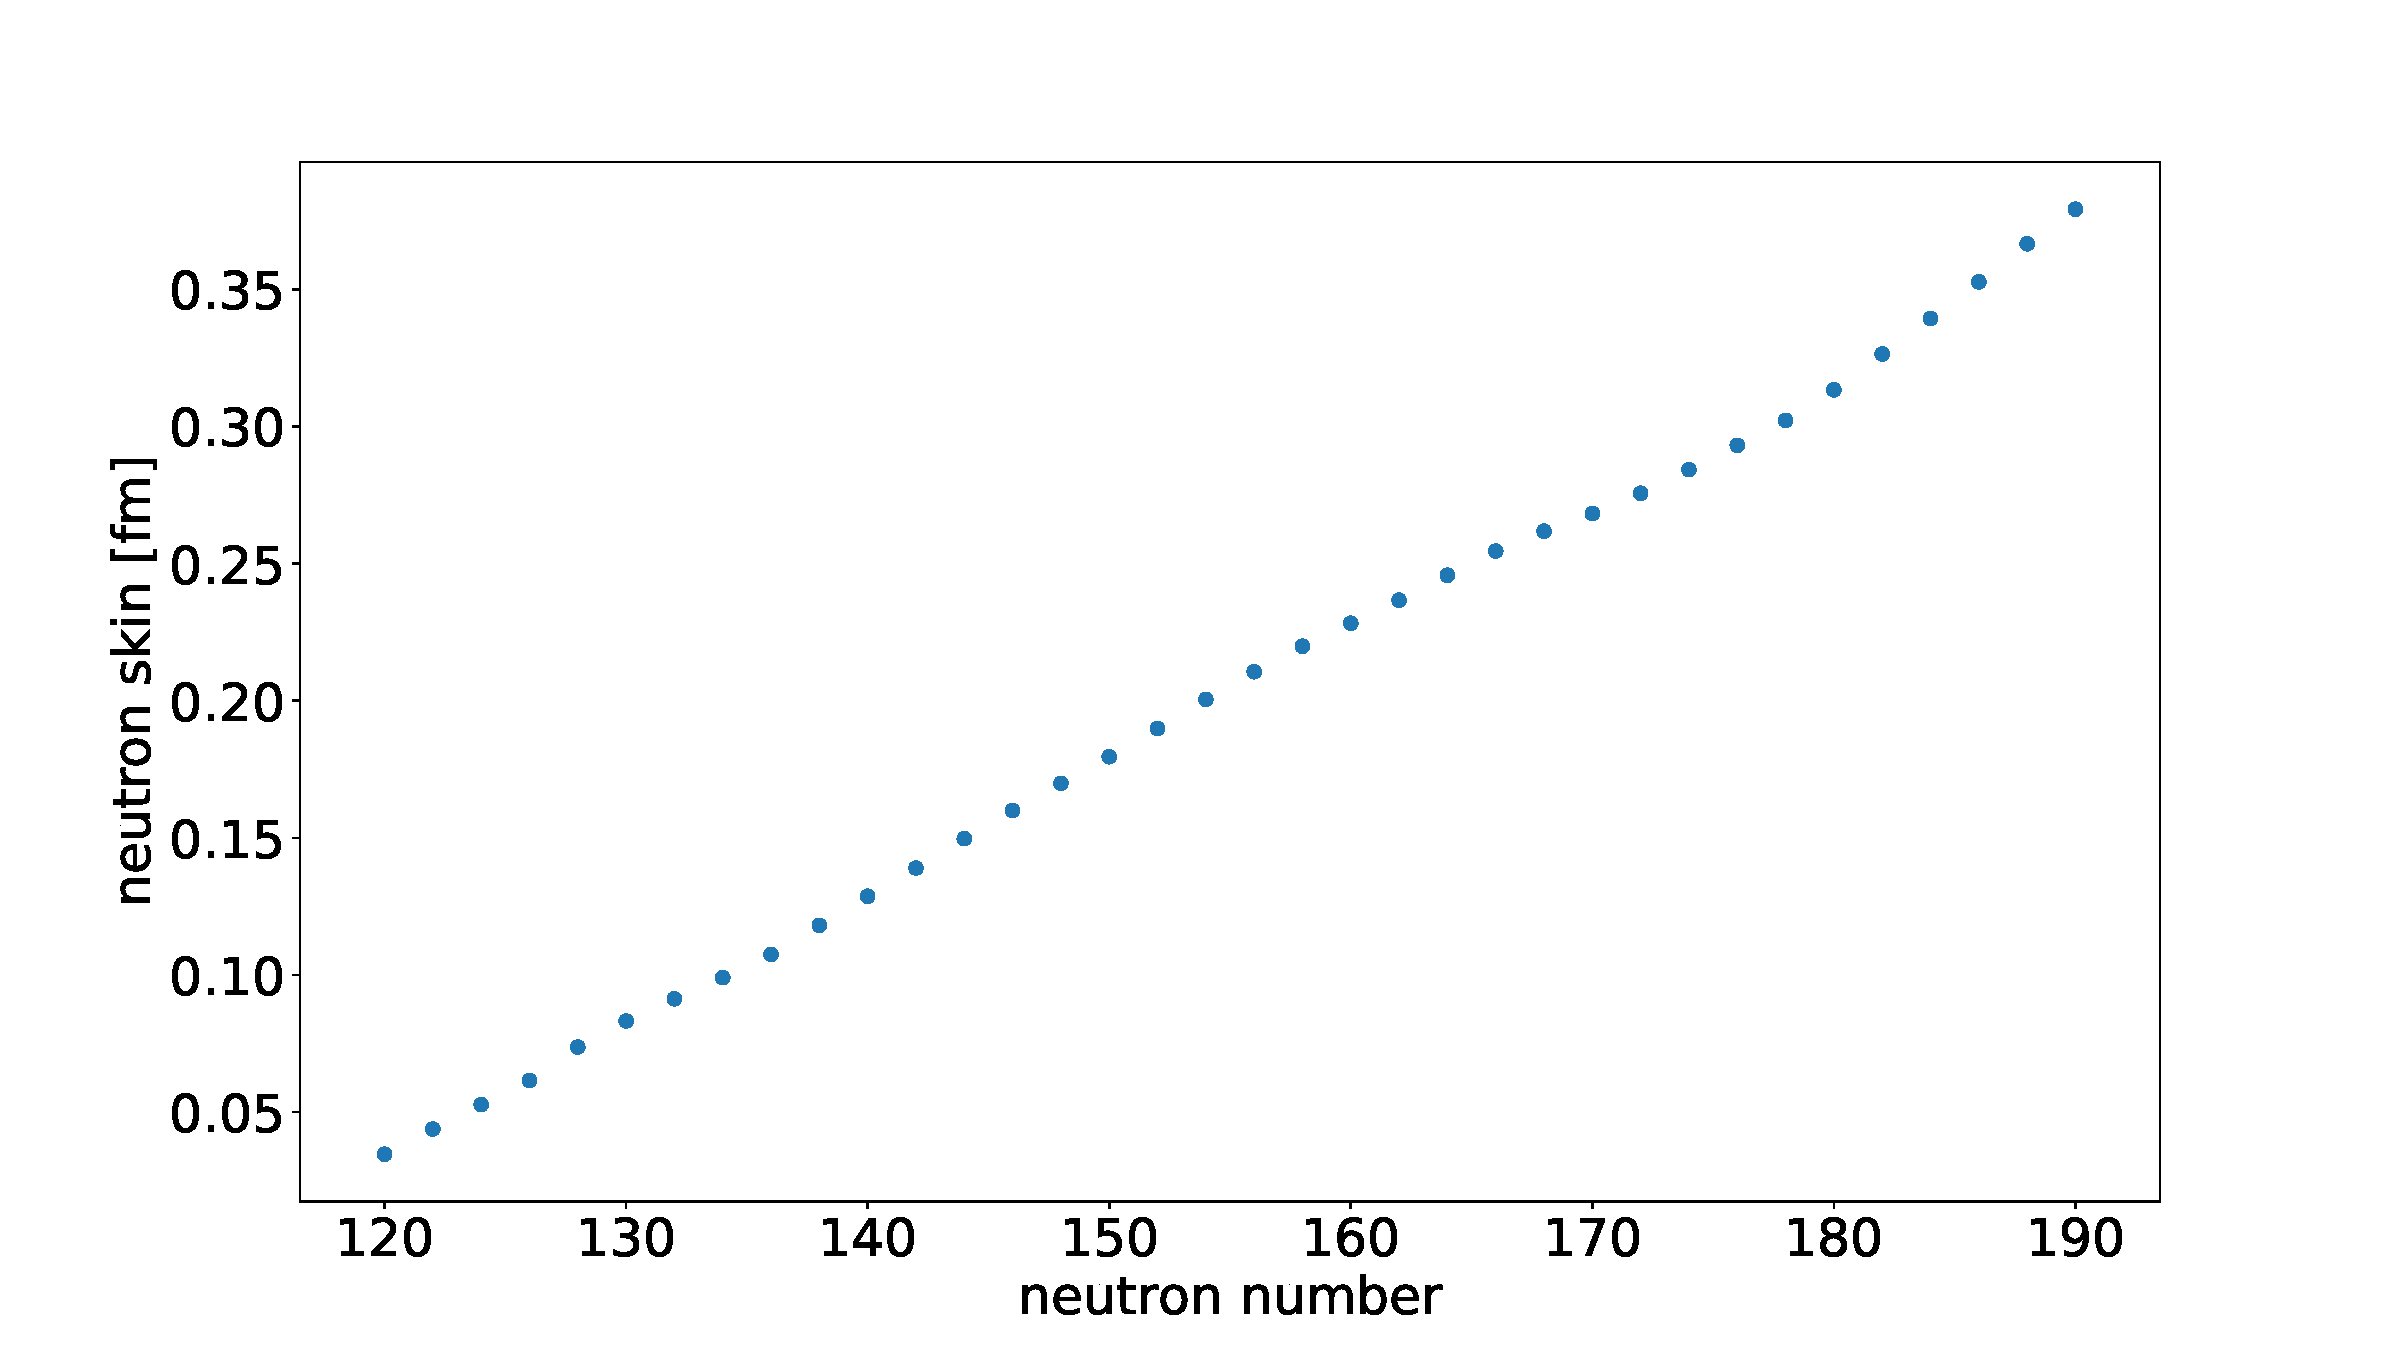
\includegraphics[width=1.1\textwidth]{skin.pdf}
    \end{textblock*}
    \begin{textblock*}{0.5\paperwidth}(0.48\paperwidth,0.3\paperheight)
        \centering
        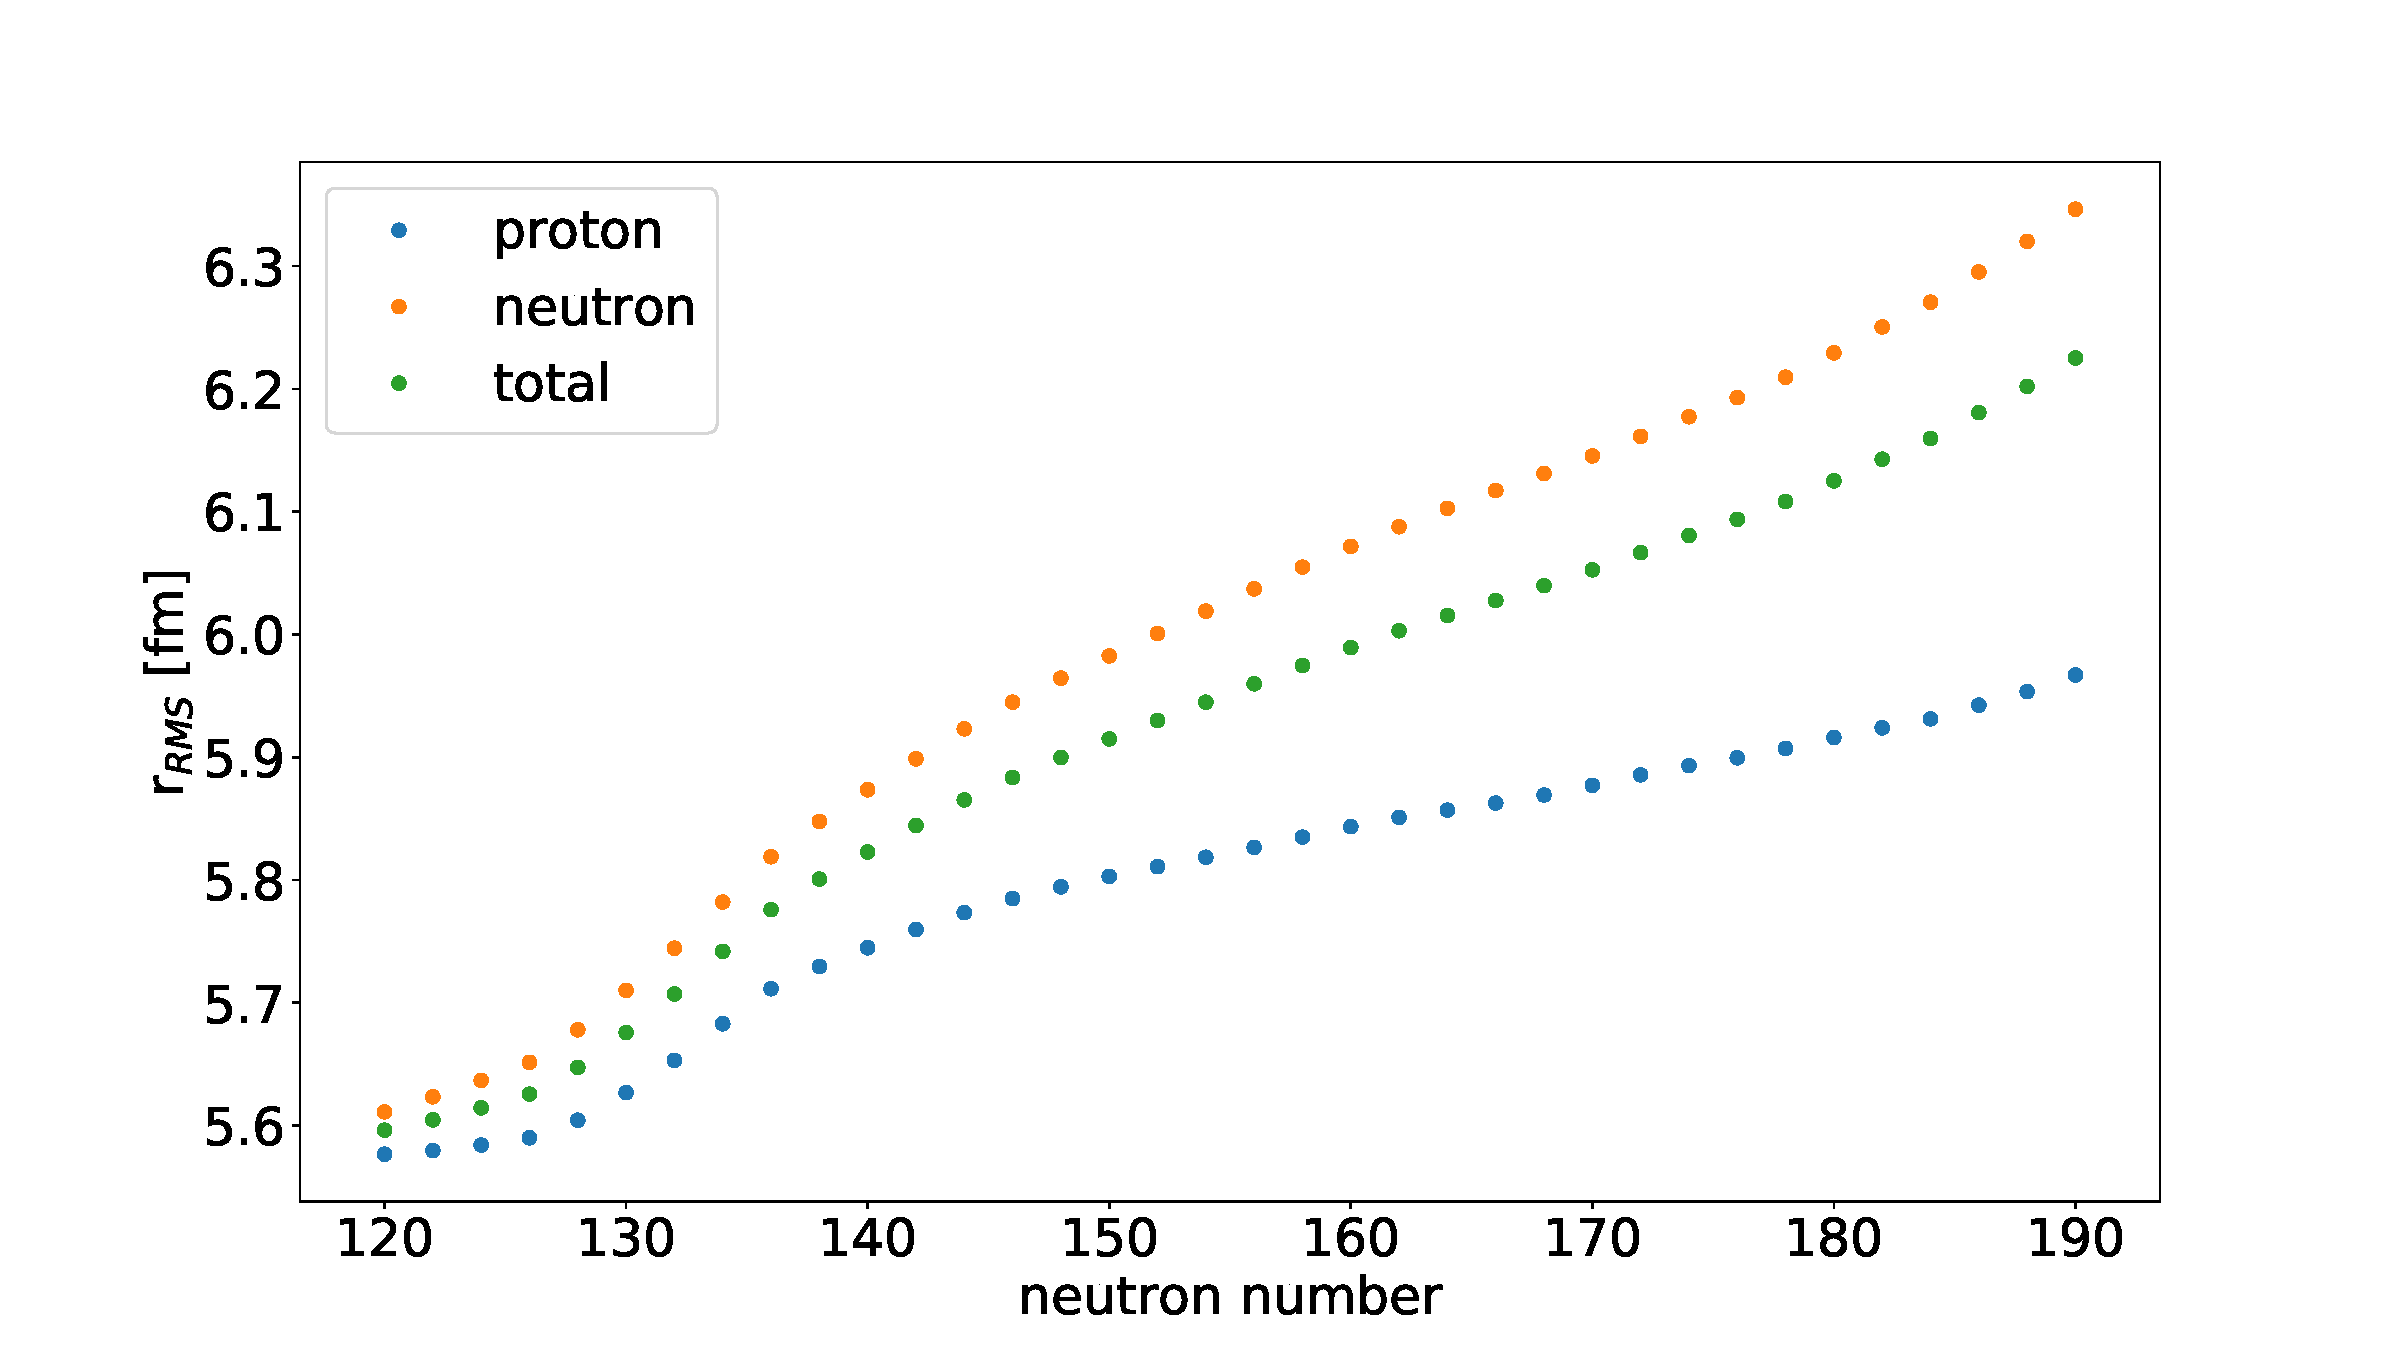
\includegraphics[width=1.1\textwidth]{totalrms.pdf}
    \end{textblock*}
    \begin{textblock*}{0.6\paperwidth}(0.2\paperwidth,0.25\paperheight)
            Neutron skin increasing for neutron rich nuclei
    \end{textblock*}

\end{frame}

\begin{frame}{rms for prolate and oblate configurations}

    \centering 
    \begin{textblock*}{0.8\paperwidth}(0.1\paperwidth,0.1\paperheight)
        \centering
        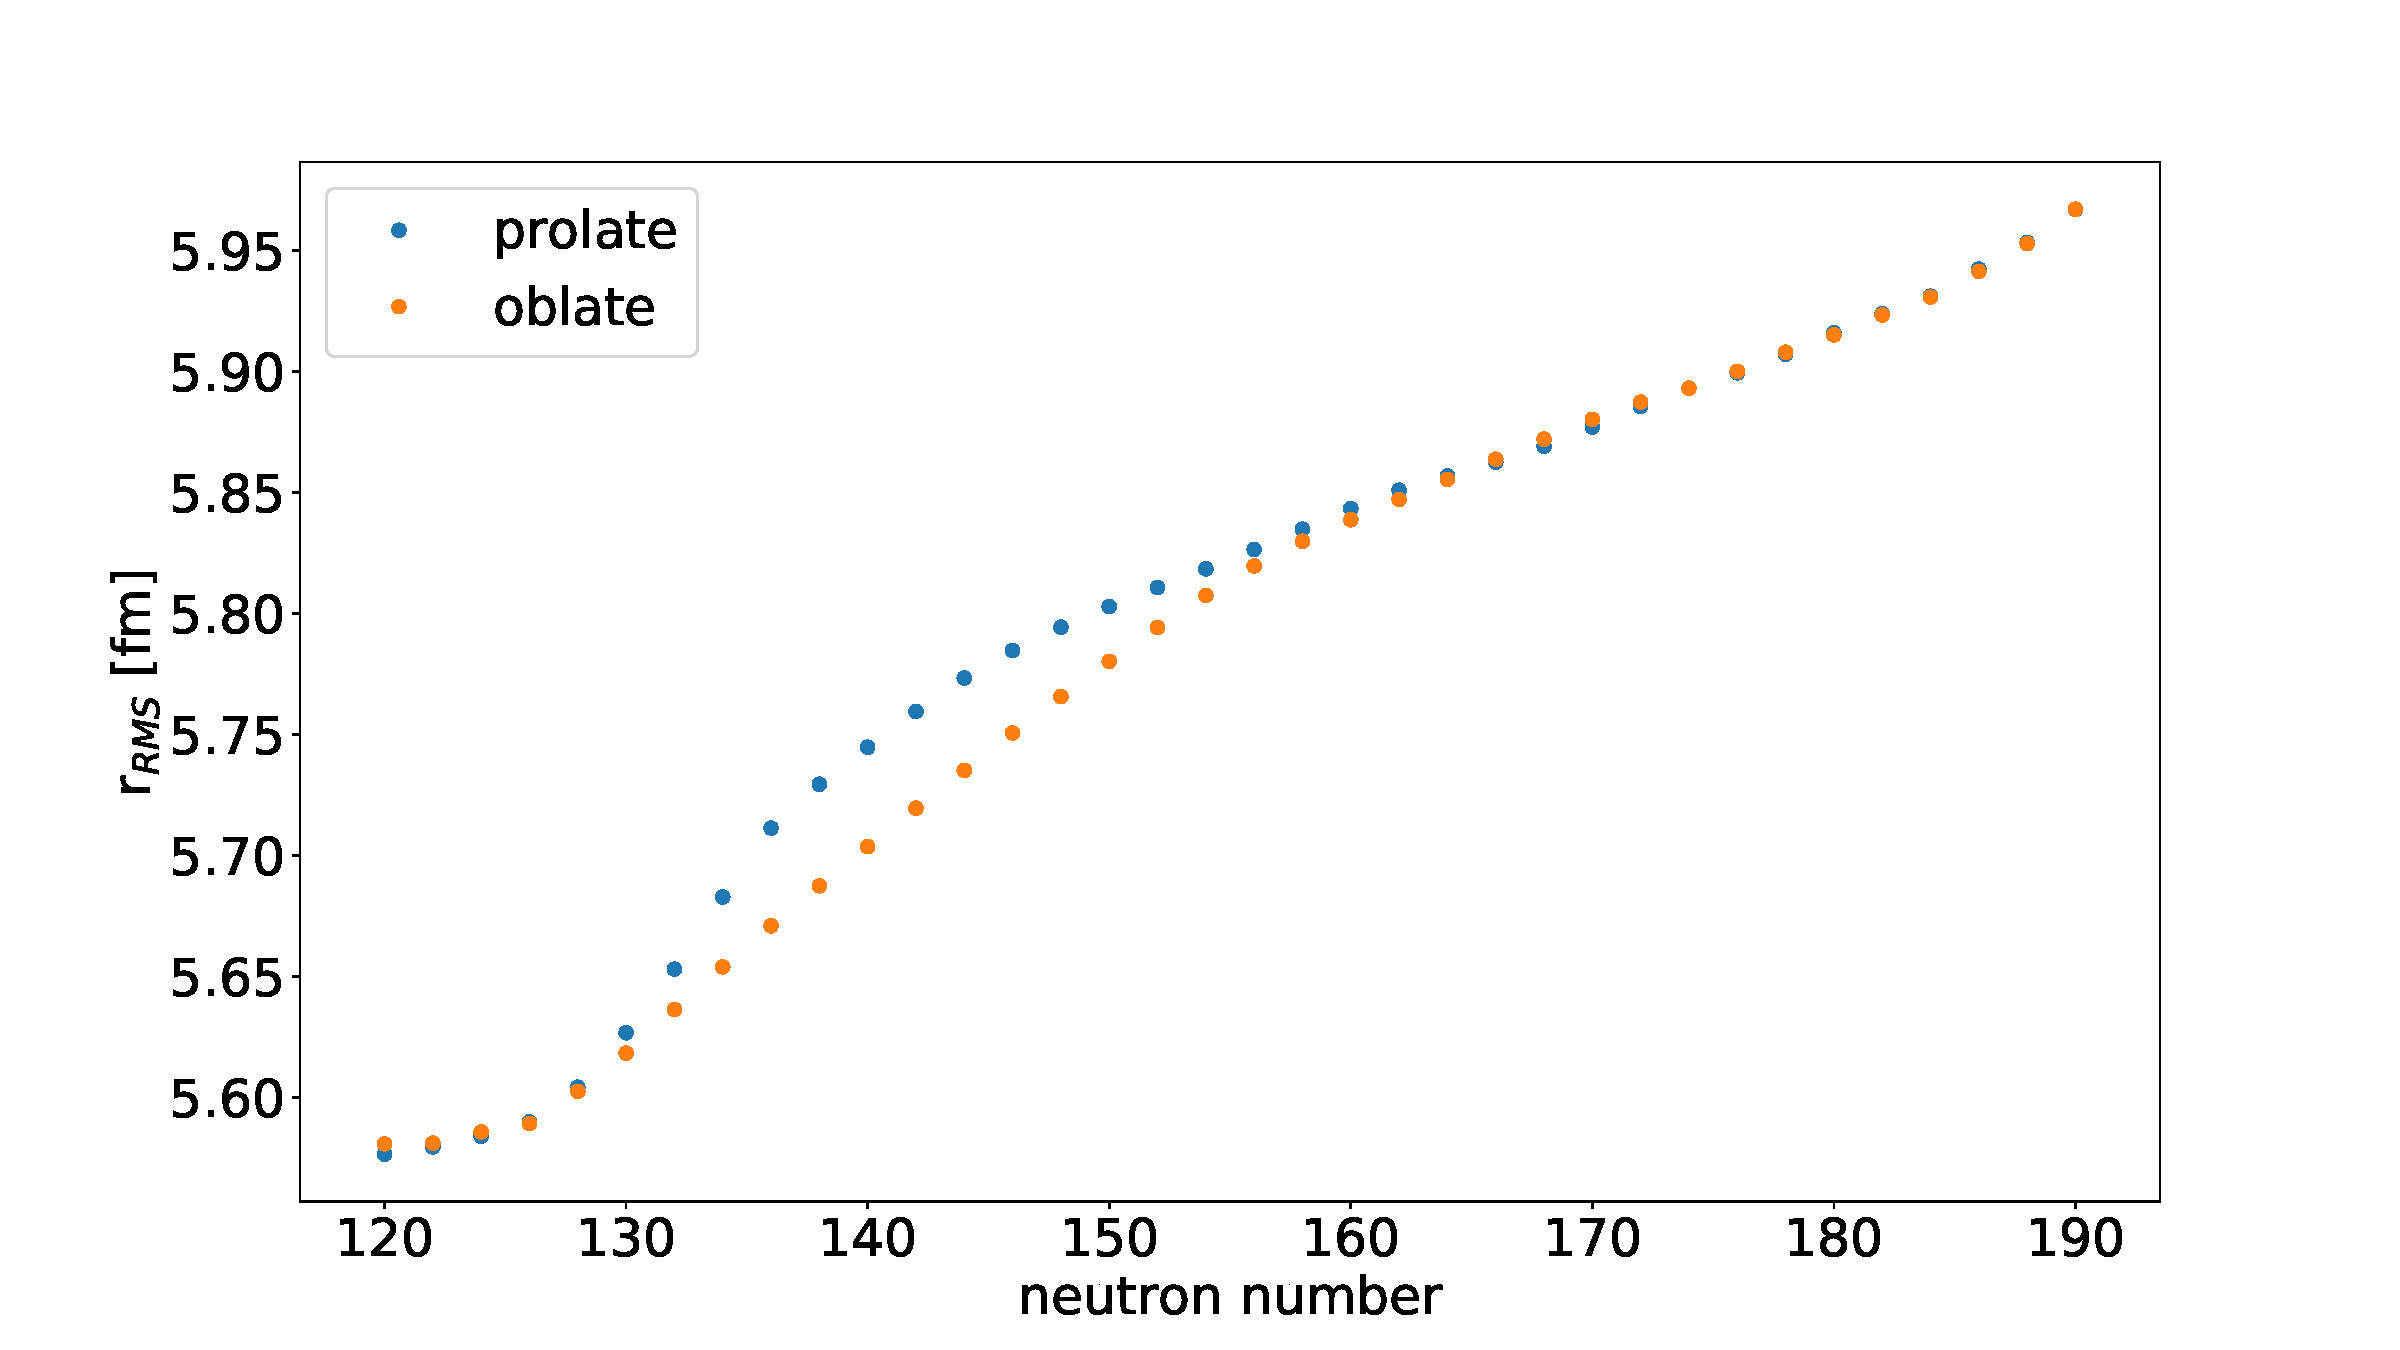
\includegraphics[width=1.\textwidth]{rms_comparison.pdf}
    \end{textblock*}

\end{frame}


\begin{SectionTitle}
	\begin{frame}
		\begin{textblock*}{0.5\paperwidth}(0.25\paperwidth,0.25\paperheight)
			\centering
			\textbf{\LARGE Ion Beam Simulation}
		\end{textblock*}
		\begin{textblock*}{0.5\paperwidth}(0.25\paperwidth,0.4\paperheight)
			\centering
			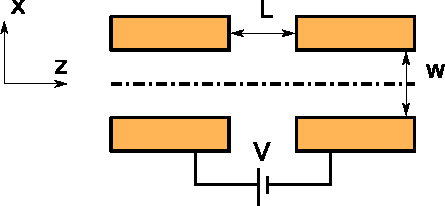
\includegraphics[width=.8\textwidth]{ibs_logo.pdf}
		\end{textblock*}
	\end{frame}
 \end{SectionTitle}

\begin{frame}{SIMION Simulations}
    \begin{textblock*}{0.5\paperwidth}(0.48\paperwidth,0.4\paperheight)
        \centering
        \begin{itemize}
            \item Professional software package
            \item Used to calculate electric fields and the trajectories of charged particles in those fields
            \item Electrostatic fields can be modelled as boundary value problem solutions of an elliptical partial differential equation (Laplace equation)
        \end{itemize}
    \end{textblock*}
    \begin{textblock*}{0.43\paperwidth}(0.05\paperwidth,0.2\paperheight)
			\centering
			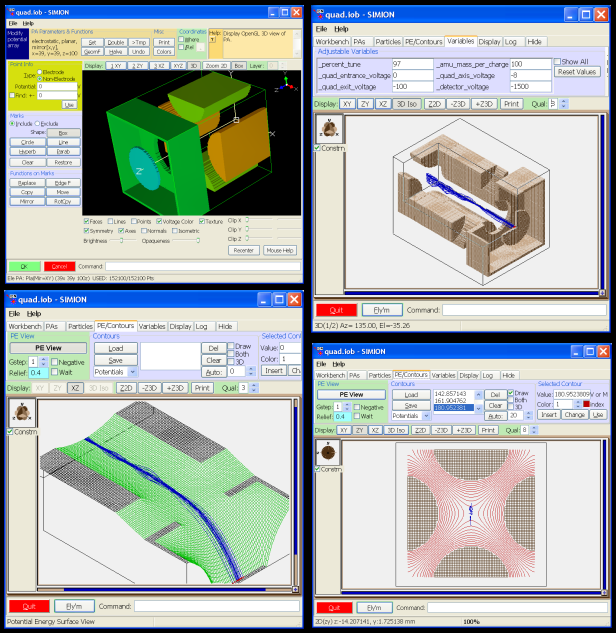
\includegraphics[width=.9\textwidth]{Simion.png}
		\end{textblock*}
  
\end{frame}


\begin{frame}{SIMION Simulations}
    \begin{textblock*}{0.5\paperwidth}(0.5\paperwidth,0.4\paperheight)
        \centering
        \begin{itemize}
            \item Flying 1000 ions
            \item Circle distribution start point along x-axis
            \item Cone direction distribution (5°) along z-axis
            \item Kinetic energy 10keV, acceleration of 10keV
            \item Extract $x_i$, $x_i'$, $x_f$, $x_f'$ for each ion
        \end{itemize}
    \end{textblock*}
    \begin{textblock*}{0.5\paperwidth}(0.02\paperwidth,0.3\paperheight)
			\centering
			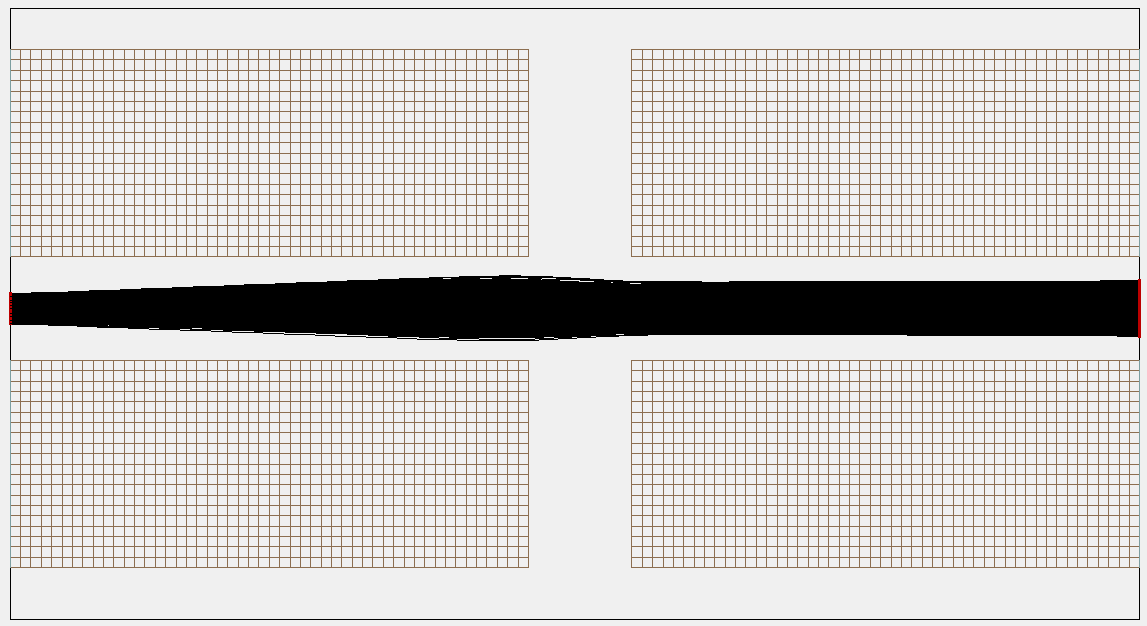
\includegraphics[width=.9\textwidth]{SimionScreenshot.png}
		\end{textblock*}
  
\end{frame}

\begin{frame}{Description of Transfer Matrix}
    \begin{textblock*}{0.5\paperwidth}(0.425\paperwidth,0.2\paperheight)
        \centering
        \begin{equation*}
            \begin{pmatrix}x_f \\ x_f'\end{pmatrix} = M_\text{drift  } M_\text{gap  } M_\text{drift  } \cdot \begin{pmatrix}x_i \\ x_i'\end{pmatrix}
        \end{equation*}
        
        \begin{equation*}
            \begin{pmatrix}x_f \\ x_f'\end{pmatrix} = \begin{pmatrix} a_{11} & a_{12}\\  a_{21} & a_{22}\end{pmatrix} \cdot \begin{pmatrix}x_i \\ x_i'\end{pmatrix}
        \end{equation*}

        \begin{equation}
            x_f = a_{11} x_i +  a_{12} x'_i  
        \end{equation}
        \begin{equation}
            x_f' = a_{21} x_i +  a_{22} x'_i 
        \end{equation}
            
    \end{textblock*}
    \begin{textblock*}{0.5\paperwidth}(0.\paperwidth,0.35\paperheight)
			\centering
			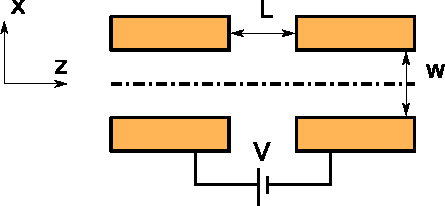
\includegraphics[width=.8\textwidth]{ibs_logo.pdf}
		\end{textblock*}
  
\end{frame}

\begin{frame}{Extraction of Transfer Matrix Elements $a_{ij}$}
    \begin{textblock*}{0.5\paperwidth}(0.02\paperwidth,0.25\paperheight)
			\centering
			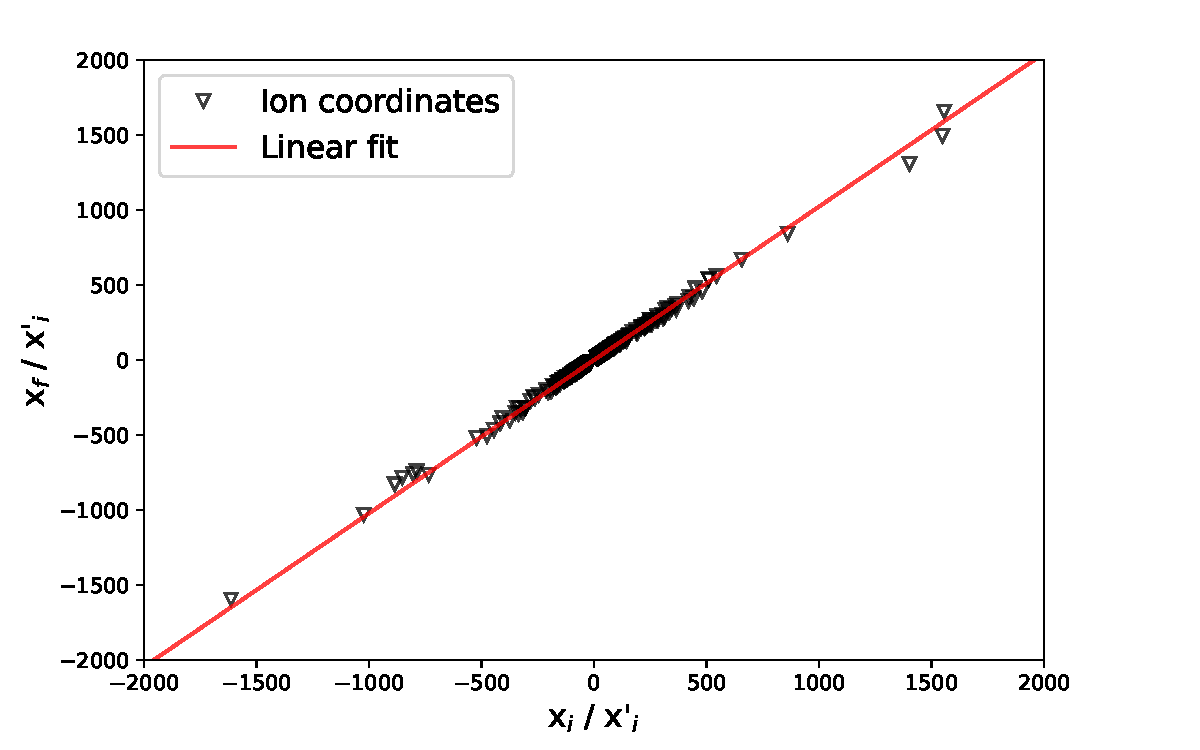
\includegraphics[width=.9\textwidth]{FirstCoord_Eq.pdf}
            \begin{equation*}
                \frac{x_f}{x_i'} = a_{11}\frac{x_i}{x_i'} + a_{12}
            \end{equation*}
		\end{textblock*}
    \begin{textblock*}{0.5\paperwidth}(0.52\paperwidth,0.25\paperheight)
			\centering
			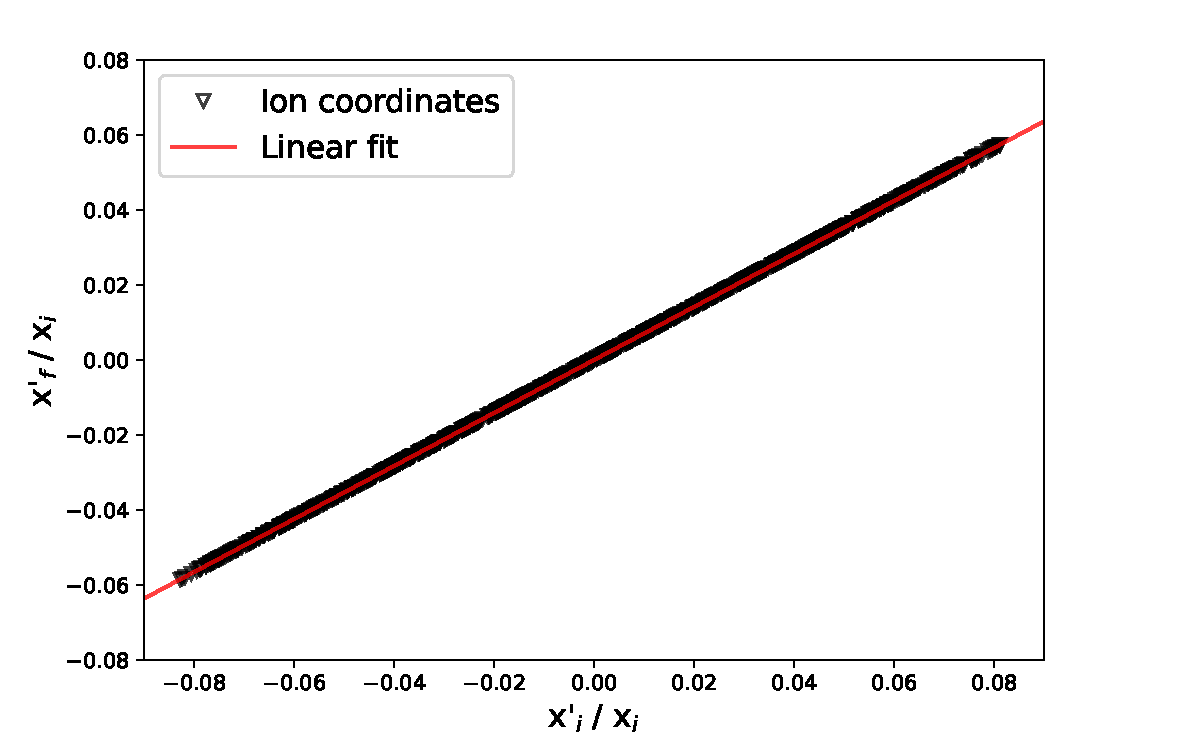
\includegraphics[width=.9\textwidth]{SecondCoord_Eq.pdf}
            \begin{equation*}
                \frac{x_f'}{x_i} = a_{22}\frac{x_i'}{x_i} + a_{21}
            \end{equation*}
		\end{textblock*}
  
\end{frame}


\begin{frame}{Transfer Matrix Calculation}
    \begin{textblock*}{0.5\paperwidth}(0.425\paperwidth,0.2\paperheight)
        \centering
        \begin{equation*}
            \begin{pmatrix}x_f \\ x_f'\end{pmatrix} = M_\text{drift  } M_\text{gap  } M_\text{drift  } \cdot \begin{pmatrix}x_i \\ x_i'\end{pmatrix}
        \end{equation*}
        Drift matrix $M_\text{drift  }$: 
        \begin{equation*}
            \begin{pmatrix}x_f \\ x_f'\end{pmatrix} \xrightarrow{\text{Drift length tube S}} \begin{pmatrix} x_f + x_f' S \\ x_f'\end{pmatrix}
        \end{equation*}

        \begin{equation*}
            M_\text{drift  } = \begin{pmatrix} 1 & S \\ 0 & 1 \end{pmatrix}, \quad  M_\text{drift  }^{-1} = \begin{pmatrix} 1 & -S \\ 0 & 1 \end{pmatrix}
        \end{equation*}

            
    \end{textblock*}
    \begin{textblock*}{0.5\paperwidth}(0.\paperwidth,0.35\paperheight)
		\centering
		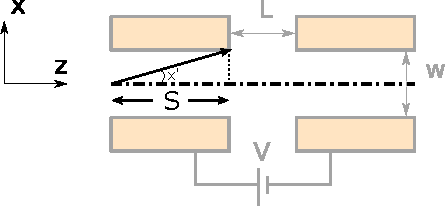
\includegraphics[width=.8\textwidth]{ibs_logo_2.pdf}
	\end{textblock*}

\end{frame}

\begin{frame}{Transfer Matrix Calculation}
    \begin{textblock*}{0.5\paperwidth}(0.425\paperwidth,0.27\paperheight)
        \centering
        Result from fit to simulation Ddata:
        \begin{equation*}
            M_\text{drift  } M_\text{gap  } M_\text{drift  } = \begin{pmatrix} 1.022 & 0.151 \\ \approx 0 & 0.707 \end{pmatrix}
        \end{equation*}

        with drift Length $S=50$\,mm

         \vspace{0.1\paperheight}
        
        Multiplying with $M_\text{drift  }^{-1}$ from both sides yields: 

        \begin{equation*}
            M_\text{gap  } = \begin{pmatrix} 1.022 & -86.310  \\ \approx 0 & 0.707 \end{pmatrix}
        \end{equation*}

            
    \end{textblock*}
    \begin{textblock*}{0.5\paperwidth}(0.\paperwidth,0.35\paperheight)
		\centering
		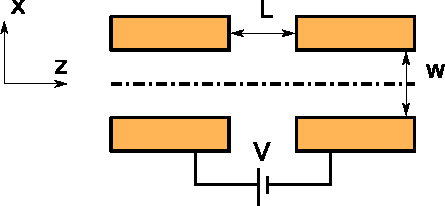
\includegraphics[width=.8\textwidth]{ibs_logo.pdf}
	\end{textblock*}
  

\end{frame}

\end{document}